
% To do: Check optimilaity claims

\documentclass{IEEEtran}

%
% If IEEEtran.cls has not been installed into the LaTeX system files,
% manually specify the path to it like:
% \documentclass[10pt,journal,compsoc]{../sty/IEEEtran}


% Some very useful LaTeX packages include:
% (uncomment the ones you want to load)


% *** MISC UTILITY PACKAGES ***
%
%\usepackage{ifpdf}
% Heiko Oberdiek's ifpdf.sty is very useful if you need conditional
% compilation based on whether the output is pdf or dvi.
% usage:
% \ifpdf
%   % pdf code
% \else
%   % dvi code
% \fi
% The latest version of ifpdf.sty can be obtained from:
% http://www.ctan.org/tex-archive/macros/latex/contrib/oberdiek/
% Also, note that IEEEtran.cls V1.7 and later provides a builtin
% \ifCLASSINFOpdf conditional that works the same way.
% When switching from latex to pdflatex and vice-versa, the compiler may
% have to be run twice to clear warning/error messages.

\usepackage{upgreek}
% *** CITATION PACKAGES ***
%
\ifCLASSOPTIONcompsoc
  % IEEE Computer Society needs nocompress option
  % requires cite.sty v4.0 or later (November 2003)
  \usepackage[nocompress]{cite}
\else
  % normal IEEE
  \usepackage{cite}
\fi


% cite.sty was written by Donald Arseneau
% V1.6 and later of IEEEtran pre-defines the format of the cite.sty package
% \cite{} output to follow that of IEEE. Loading the cite package will
% result in citation numbers being automatically sorted and properly
% "compressed/ranged". e.g., [1], [9], [2], [7], [5], [6] without using
% cite.sty will become [1], [2], [5]--[7], [9] using cite.sty. cite.sty's
% \cite will automatically add leading space, if needed. Use cite.sty's
% noadjust option (cite.sty V3.8 and later) if you want to turn this off
% such as if a citation ever needs to be enclosed in parenthesis.
% cite.sty is already installed on most LaTeX systems. Be sure and use
% version 5.0 (2009-03-20) and later if using hyperref.sty.
% The latest version can be obtained at:
% http://www.ctan.org/tex-archive/macros/latex/contrib/cite/
% The documentation is contained in the cite.sty file itself.
%
% Note that some packages require special options to format as the Computer
% Society requires. In particular, Computer Society  papers do not use
% compressed citation ranges as is done in typical IEEE papers
% (e.g., [1]-[4]). Instead, they list every citation separately in order
% (e.g., [1], [2], [3], [4]). To get the latter we need to load the cite
% package with the nocompress option which is supported by cite.sty v4.0
% and later. Note also the use of a CLASSOPTION conditional provided by
% IEEEtran.cls V1.7 and later.
% *** GRAPHICS RELATED PACKAGES ***
%
\ifCLASSINFOpdf
   \usepackage[pdftex]{graphicx}
   \usepackage{subfigure}
  % declare the path(s) where your graphic files are
  % \graphicspath{{../pdf/}{../jpeg/}}
  % and their extensions so you won't have to specify these with
  % every instance of \includegraphics
  % \DeclareGraphicsExtensions{.pdf,.jpeg,.png}
\else
  % or other class option (dvipsone, dvipdf, if not using dvips). graphicx
  % will default to the driver specified in the system graphics.cfg if no
  % driver is specified.
   \usepackage[dvips]{graphicx}
   \usepackage{subfigure}
  % declare the path(s) where your graphic files are
  % \graphicspath{{../eps/}}
  % and their extensions so you won't have to specify these with
  % every instance of \includegraphics
  % \DeclareGraphicsExtensions{.eps}
\fi


% graphicx was written by David Carlisle and Sebastian Rahtz. It is
% required if you want graphics, photos, etc. graphicx.sty is already
% installed on most LaTeX systems. The latest version and documentation
% can be obtained at: 
% http://www.ctan.org/tex-archive/macros/latex/required/graphics/
% Another good source of documentation is "Using Imported Graphics in
% LaTeX2e" by Keith Reckdahl which can be found at:
% http://www.ctan.org/tex-archive/info/epslatex/
%
% latex, and pdflatex in dvi mode, support graphics in encapsulated
% postscript (.eps) format. pdflatex in pdf mode supports graphics
% in .pdf, .jpeg, .png and .mps (metapost) formats. Users should ensure
% that all non-photo figures use a vector format (.eps, .pdf, .mps) and
% not a bitmapped formats (.jpeg, .png). IEEE frowns on bitmapped formats
% which can result in "jaggedy"/blurry rendering of lines and letters as
% well as large increases in file sizes.
%
% You can find documentation about the pdfTeX application at:
% http://www.tug.org/applications/pdftex
% *** MATH PACKAGES ***
%
\usepackage[cmex10]{amsmath}
\usepackage{amssymb}
 \usepackage{graphicx}
  \usepackage{tabulary}
  \usepackage{array,booktabs,longtable,tabularx}
% A popular package from the American Mathematical Society that provides
% many useful and powerful commands for dealing with mathematics. If using
% it, be sure to load this package with the cmex10 option to ensure that
% only type 1 fonts will utilized at all point sizes. Without this option,
% it is possible that some math symbols, particularly those within
% footnotes, will be rendered in bitmap form which will result in a
% document that cannot be IEEE Xplore compliant!
%
% Also, note that the amsmath package sets \interdisplaylinepenalty to 10000
% thus preventing page breaks from occurring within multiline equations. Use:
%\interdisplaylinepenalty=2500
% after loading amsmath to restore such page breaks as IEEEtran.cls normally
% does. amsmath.sty is already installed on most LaTeX systems. The latest
% version and documentation can be obtained at:
% http://www.ctan.org/tex-archive/macros/latex/required/amslatex/math/
% *** SPECIALIZED LIST PACKAGES ***
%
\usepackage[justification=centering]{caption}
\usepackage{url}
\usepackage{amsmath}
\usepackage{amsfonts}
\newtheorem{definition}{\noindent{\bf Definition}}
\newtheorem{lemma}{\noindent{\bf Lemma}}
\newtheorem{theorem}{\noindent{\bf Theorem}}
\newtheorem{proposition}{\noindent{\bf proposition}}



\usepackage{algorithm}
\usepackage{algorithmic}
% algorithmic.sty was written 







\begin{document}

\title{ Yosemite: Efficient Scheduling of Weighted Coflows in Data Centers}
%\author{\IEEEauthorblockN{Han Zhang\IEEEauthorrefmark{1}\IEEEauthorrefmark{3},  Xingang Shi\IEEEauthorrefmark{2}\IEEEauthorrefmark{3}, Xia Yin\IEEEauthorrefmark{1}\IEEEauthorrefmark{3}, Zhiliang Wang\IEEEauthorrefmark{2}\IEEEauthorrefmark{3},YingYa Guo\IEEEauthorrefmark{1}\IEEEauthorrefmark{3}}
%\IEEEauthorblockA{\IEEEauthorrefmark{1}Department of Computer Science and Technology, Tsinghua University\\
%\IEEEauthorrefmark{2}Institute for Network Sciences and Cyberspace, Tsinghua University\\
%\IEEEauthorrefmark{3}Tsinghua National Laboratory for Information Science and Technology (TNLIST)\\
%Beijing, P.R. China\\
%Email:\{zhanghan, wzl, yxia,guoyingya\}@csnet1.cs.tsinghua.edu.cn, \{shixg\}@cernet.edu.cn
%}
%}
\author{Paper ID: \#117}
% make the title area
\maketitle



\begin{abstract}
Nowadays, low latency and high throughput are required by data center applications. Coflow has been proposed as a new abstraction to capture the communication patterns in a rich set of data parallel applications, so that their application-level semantics can be effectively modeled. By taking coflows, instead of flows or packets, as the basic elements in network resource allocation or scheduling, application-level optimization goals such as reducing the coflow completion time (CCT) or application transfer latency can be better achieved. Although efficient coflow scheduling methods have been studied in this aspect, in this paper, we propose {\em weighted coflows} as a further step in this direction, where weights are used to express the importance or priorities of different coflows or applications, and weighted coflow completion time (WCCT) is set as the optimization target. We design and implement Yosemite, a system that aims to minimize WCCT by dynamically scheduling coflows according to their weights and the instantaneous network condition. We test Yosemite's performance against several flow or coflow scheduling methods, by trace-driven simulations as well as real delopyment in a cloud testbed. Our trace-driven simulations show that, Yosemite's online scheduling algorithm performs about 20\%-50\% and 30\%-60\% better than that of Varys and Aalo, two state-of-the-art coflow scheduling systems, respectively. And in our testbed evaluations, Yosemite achieves 30\% average improvement against Varys.%Nowadays, applications (hadoop, ceph, etc.) in data center need network to provide them with low latency and high throughput. 
%However, as resources of data center network are limited, efficient network schedule methods are needed. Recently, the proposed
%application level abstraction coflow tries to regard flows of data-parallel applications as a whole, so that transfer latency of applications will be reduced. 
%For reducing application transfer latency, application level optimization methods perform better than flow level ones.
%This is because often a application's communication stage cannot finish until all its flows have completed. 
%Although coflow level scheduling methods such as Varys and Aalo perform well on reducing application transfer latency,
%they ignore different applications always have different level of importance and 
%scheduling just depends on network condition and characters (width, length) of coflows is not enough.
%In reality, the importance of applications should also be taken into consideration.
%In this paper, we incorporate weight to present the importance of applications and try to minimize average coflow weight completion time.
%To achieve this, we design Yosemite-a system that aims to minimize average weight coflow completion time.
%We test Yosemite's performance in trace-driven simulation as well as our cloud platform and then compare its performance with state-of-art methods.  
%Trace-driven simulation shows that Yosemite performs about 20\%$\sim$50\%better than Varys and 30\%$\sim$60\% better than Aalo. 
%Testbed evaluation shows Yosemite performs  30\% and 35\% better than Varys and Aalo respectively on average.
\end{abstract}

\section{Introduction}\label{introduction}

Nowadays, low latency\cite{Latency}\cite{munir2014friends} and high throughput\cite{CloudMirror} are required by data center applications, for example, 
those with map-reduce style data-intensive computing \cite{dean2008mapreduce}, and those using distributed file storgage\cite{lin2010secure}\cite{dimakis2006decentralized}, etc.
To meet these requirements, the data center networking infrastructure has been specially tailored, with a tremendous amount of efforts to improve the network topology and routing, as well as the transportation. 

Among these efforts, flow level scheduling methods try to schedule arriving packets according to the characteristics of the corrsponding flows. For example, PDQ\cite{PDQ} and pFabric\cite{pFabric} approximate the {\em shortest job first} (SJF) policy to let shorter flows preempt the bandwidth of longer ones. 
As a result, the average flow completion time (FCT) tends to be reduced, so does applications' transport latency. 
However, flow level scheduling methods still have several deficiencies\cite{chowdhury2011managing}. 
On the one hand, flow level scheduling has to be carried out quite frequently, such that centralized scheduler may face huge pressure on its own computation and communication, while decentralized scheduler may face worse scheduling performance.
On the other hand, some tardy flows may lag behind and affect the overall performance of an application, because the communication of the application cannot finish until all its flows have completed their transmission.

Recently, coflow has been proposed as a new abstraction to capture the communication patterns in a rich set of data parallel applications, so that their application-level semantics can be effectively modeled. 
According to \cite{chowdhury2012coflow}, a coflow is {\em a collection of flows between two groups of machines with associated semantics and a collective objective.} The collection of flows share a common performance goal, e.g., minimizing the completion time of the latest flow or ensuring that flows meet a common deadline, capturing the application-level requirements in a way better than individual flows can.
Efficient coflow scheduling methods targeting minimizing coflow completion time (CCT) have been studied. 
Varys \cite{chowdhury2014efficient} takes a coflow's network bottleneck as the most important factor that determines the coflow completion time. 
It proposes the {\em Smallest-Effective-Bottleneck-First} (SEBF) heuristic, which schedules coflows according to their bottleneck completion time. 
It also uses {\em Minimum-Allocation-for-Desired-Duration} (MADD) to compute the bandwidth that coflows deserve to get. 
Non-clairvoyant methods are also studied, including Aalo \cite{chowdhury2015efficient}, sunflows \cite{huang2016sunflow} and CODA \cite{zhang2016coda}, which do not assume the priori knowledge about a coflow's characteristics such as the number, the length, or the arrival time of its constituting flows.
Naturally, they tend to have relatively worse performance than Varys.

In this paper, we propose {\em weighted coflows} as a further step in this direction, where weights are used to express the importance or priorities of different coflows or applications in meeting a short completion time, and weighted coflow completion time (WCCT) is set as the optimization target. 
This is natural since there exist both delay sensitive and insensitive applications, and some 
applications may gain (or lose) more revenue than others in the same amount of time.
For example, supporting the internal communication requirement of a search engine with intense internal computation should be more emergent than supporting the file backup on a distributed storage system. When scheduling coflows from these two applications, we would like to take this difference into consideration and assign different weights to them, i.e., coflows of search engine have a higher weight, while coflows of file back have a lower weight.

We formulate the weighted coflow completion time optimization (WCCO) problem, and present a 2-approximate offline algorithm that borrows ideas from the concurrent open shop problem \cite{mastrolilli2010minimizing}. We then modify the algorithm to an online version, which introduces only minor performance loss compared to the offline one. 
We further design and implement Yosemite, a coflow scheduling system which is consisted of a central master node, a central monitor node, and other distributed worker nodes, and can be readily deployed in a production cloud environment like openstack. We test the performance of Yosemite by both trace-driven simulations and testbed evaluations, where Yosemite performs quite well in reducing the weighted coflow completion time. Our trace-driven simulations show that, Yosemite's online scheduling algorithm performs about 20\%$\sim$50\% and 30\%$\sim$60\% better than that of Varys and Aalo, respectively. And in our testbed evaluations, Yosemite achieves 30\%  average improvement against Varys.

Our contributions in this paper are summarized as follows:

\begin{itemize}[\IEEEsetlabelwidth{Z}]
\item We propose the weighted coflow completion time optimization (WCCO) problem and prove its equivalence to the job weighted completion time problem in the concurrent open shop setting.
\item We propose for the WCCO problem an online algorithm that performs nearly as well as a two-approximation offline algorithm.
\item We design and implement a weighted coflow scheduling system named Yosemite that is ready to be deployed in a cloud environment like openstack.  
\item We thoroughtly evaluate our scheduling algorithm and system both by simulations and testbed deployment, and show their significent performance improvement against several state-of-the-art coflow scheduling algorithms such as Varys, Aalo and Barrat.
\end{itemize}

The rest of the paper is organized as follows. In Section \ref{background} we introduce some background and the related work. 
We formulate the WCCO problem and examine its hardness in Section \ref{system model}, and propose an efficient online scheduling algorithm in Section \ref{algorithm}. 
We present the details of our Yosemite schduling system in Section \ref{Yosemite system}, 
and evalute it against several coflow schedule methods in Section \ref{evaluation}.
At last, we conclude in Section \ref{conclusion}.






\section{background and related work}\label{background}
Data center is now becoming an important infrastructure for applications. 
High throughput and low latency are required by applications.
To meet these requirements, the data center networking infrastructure has been specially tailored, 
with a tremendous amount of efforts to improve the network topology and routing, as well as the transportation.

DCTCP\cite{DCTCP}, D2TCP\cite{D2TCP}, L2DCT \cite{L2DCT} and LPD \cite{zhang2015more} emphasize on flow level scheduling. 
They propose to mark packets on a switch when instantaneous queue length exceeds a certain threshold. 
The endpoints then estimate the extent of congestion by the marked packets, and throttle flow rates in proportion to that extent. 
With the help of ECN marking mechanism, they reduce the queue length on switches, thus cutting transfer latency.
TCP-based methods are simple, 
however, they are implicit rate control method \cite{pFabric} and can never precisely estimate the right flow rates to use so as to schedule flows to minimize FCT 
while ensuring that the network is fully utilized. Then explicit methods are proposed.


D3 \cite{D3} and PDQ \cite{PDQ} can schedule flows based on some notion of urgency. 
They compute flow bandwidth according to flow deadline as well as network condition.
 A centralized controller which collects the network condition is needed. 
 Although these methods can assign rates according to flow deadlines or flows' estimated completion time, they can not satisfy the demands of applications well.
 This is because distributed applications always have many parallel flows and often an application's communication stage cannot finish until all its flows have completed.
 If we only focus on single flow scheduling, some tardy flows may finish late and it doesn't make any sense to allocate much bandwidth to the application.
 As a result, scheduling applications' flows as a whole is meaningful.
 

Until this, both the implicit and explicit methods are all flow-level optimization methods.
Having recognized limitation of flow-level methods, application level schedule methods occur. 
Barrat \cite{dogar2014decentralized}  schedules tasks in FIFO order but avoids head-of-line blocking by dynamically changing the level of multiplexing in the network. 
Using Barrat, each task has a globally unique priority-all flows within the task use this priority, irrespective of when these flows start or which part of the network they traverse. 
Barrat is simple, but for some large coflow, it can down many smaller ones. 
Varys \cite{chowdhury2014efficient} regards applications' parallel flows as coflow and it uses SEBF to schedule coflows and MADD to perform rate control, 
as a result, other coexisting coflows can make progress and the average CCT decreases.
Varys is a Clairvoyant schedule method, which means some coflow information such as coflow length and coflow width should be known beforehand.
Unfortunately, in many cases, coflow characteristics are unknown a priori and this will limit the its utilization.
To overcome this, some non-Clairvoyant methods like Aalo\cite{luo2016towards} ,sunflows\cite{ huang2016sunflow},
D-CLAS\cite{chowdhury2015efficient} and CODA \cite{zhang2016coda} do not need to know coflow information beforehand. 
They use  information accumulation or machine learning to "guess" the characters of coflow. 
Non-Clairvoyant methods can be used more widely, however, they tend to have relatively worse performance than Varys.
Although coflow level scheduling methods such as Varys and Aalo perform well on reducing application transfer latency, 
they ignore applications always have different level of importance and just scheduling depends on network condition and characters 
of coflows such as coflow length as well as width is not enough. In reality, the importance of applications should also be taken into consideration.

Some theory papers such as \cite{qiu2015minimizing} set weight to coflow to minimize average weighted coflow completion time. 
We think this is good direction as they take this difference into consideration.
However, methods such as  \cite{qiu2015minimizing} will solve complex equations which make them too complex to use in practice.
%Due to these deficiencies, in this paper, we follow this direction and  proposal 
%There are many methods to present the semantics of the application. 
%Some flow-level algorithms such as D2TCP\cite{D2TCP} and LPD\cite{zhang2015more} use deadline to present the emergency of applications. 
%Flow missing deadline will be threw way. Deadline can guarantee the application to have low bound of bandwidth and it can describe the semantics of application to some extent. 
%However, in data center network, applications do not need a minimum bandwidth or have a strict finish time constraints. 
%They just have higher level of emergency and hope to finish as quickly as possible, so another kind of method to present the emergency of application according to the semantics is needed. \cite{qiu2015minimizing} and \cite{qiu2016experimental} incorporate weight into consideration. 
%They set larger weight to the more emergency jobs. Instead of minimizing coflow completion time, t
%hey try to minimize weight coflow completion time. Comparing with optimizing weight completion time, optimizing weight completion time considers application semantics. 
%They make progress on application bandwidth allocation. However both \cite{qiu2015minimizing} and \cite{qiu2016experimental}
%have high complexity, which make them hard to deploy in practice. In reality, we need the method to compute quickly to react the burst of flows in data center network.  


\section{system model and problem formulation}\label{system model}
In this part, we define Weighted Coflow Completion Optimization (WCCO) problem and prove its equivalent to
the weighted job completion optimization in concurrent open shop\cite{roemer2006note}.

\subsection{Data center non-blocking model}

%\begin{figure}[b]
%\begin{center}
%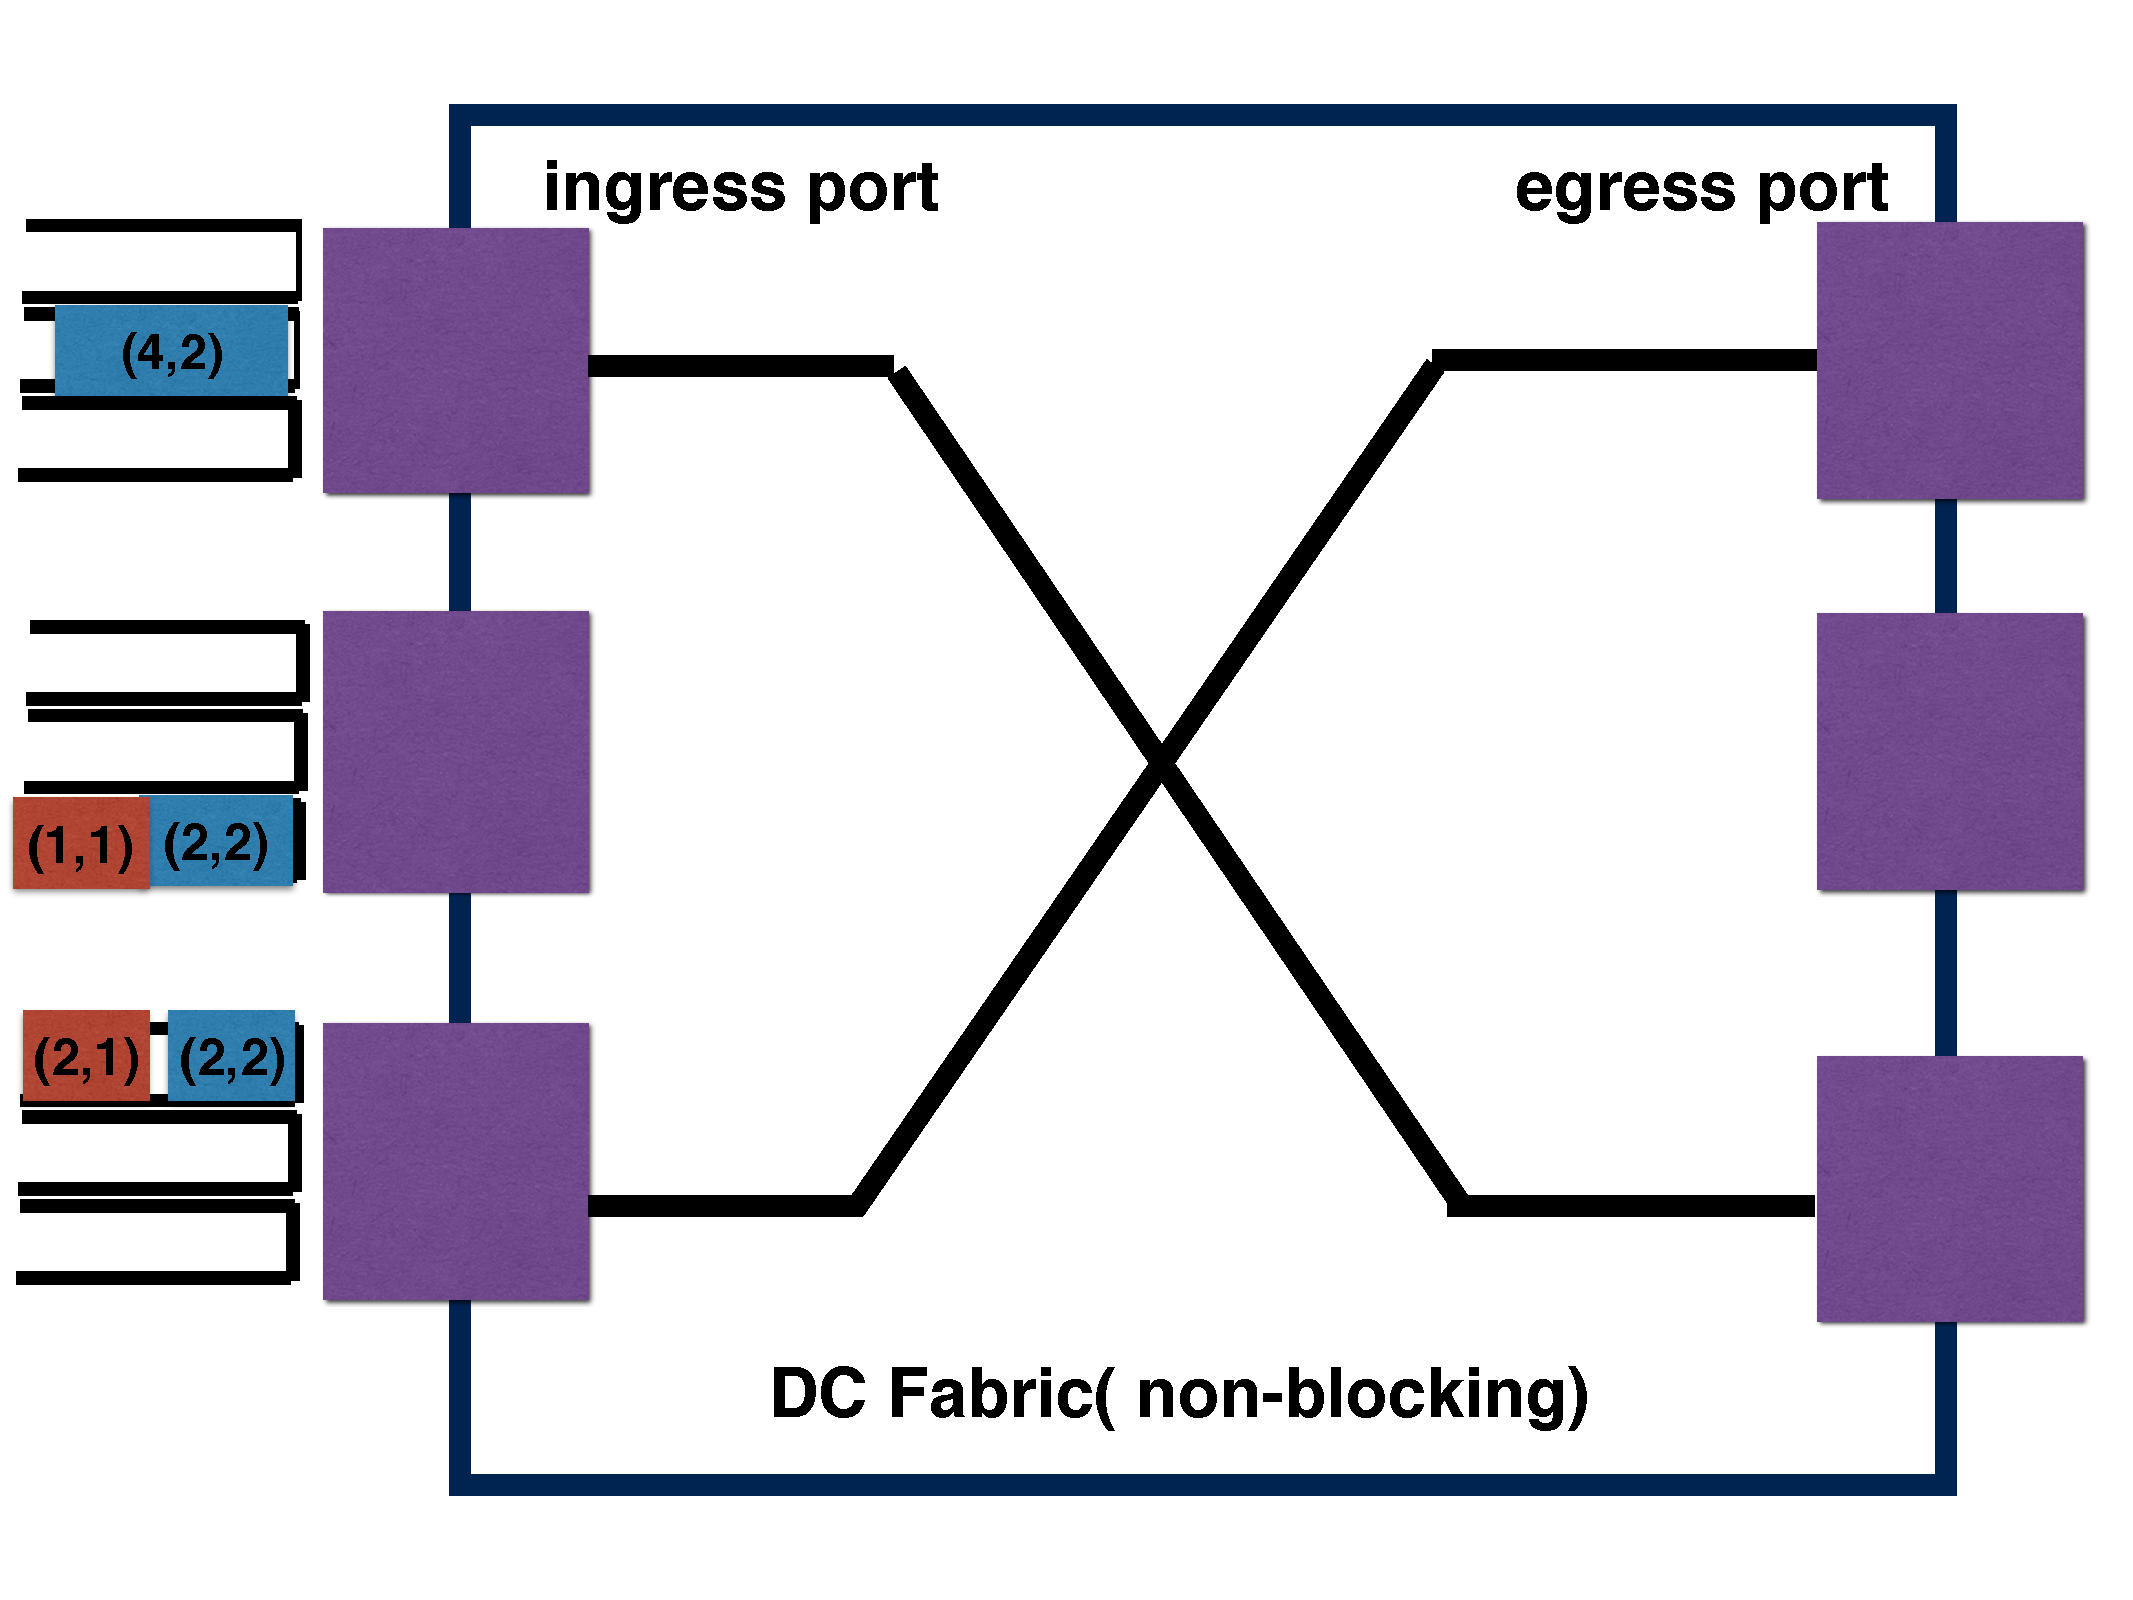
\includegraphics [width=0.8\columnwidth] {./figs/background/non_blcoking.pdf}
%\caption{Data center as non-blocking fabric: in this fabric, congestion only occurs at the ingress ports or egress ports}
%\label{Datacenter-nonblocking-fig}
%\end{center}
%\end{figure}


Recent researches\cite{chowdhury2015efficient}\cite{huang2016sunflow}\cite{chowdhury2014efficient}\cite{pFabric}  
regard  the data center network as  a big giant non-blocking switch which interconnects all the machines.
In this model all machines' ports have the same normalized unit capacity, and bandwidth compete bandwidth only at ingress and egress ports. 
Such an abstraction is reasonable and matches with recent full bisection bandwidth topologies widely used in current production data centers -
To provide uniform high capacity as well as other targets like equidistant endpoints with network core, unlimited workload mobility, etc., 
today's production data center networks widely adopt non-blocking Clos topologies by design \cite{luo2016towards}. In this paper, we believe 
data center is a non-blocking giant switch and only consider congestion at the ingress and egress ports.

\subsection{Why we choose weight}
Applications in data center have to contend with each others for limited network resources.
The state-of-art schedule methods use coflows as the abstraction to capture the communication patterns in a rich set of data parallel applications,
so that their application-level semantics can be effectively modeled.
However, applications in data center have different level of importance, 
scheduling just depends on network condition as well as the physical property of coflows is not enough.
We have to differentiate applications to satisfy their demands for bandwidth.

Some previous study\cite{D2TCP}\cite{D3}\cite{zhang2015more} use deadline to express the emergency of applications,
applications have different deadlines, thus bandwidth.
However, in reality, many applications just have different importance and do not have to finish before particular time points,
so that we abandon deadline to present the importance of applications.
In this paper, we use weight to express the importance of applications.
For the example supporting the internal communication requirement of a search engine with intense internal computation should be more emergent than supporting the file backup on a distributed storage system. 
When scheduling coflows from these two applications, we would like to take this difference into consideration and assign different weights to them, i.e., coflows of search engine have a higher weight, while coflows of file back have a lower weight.
In this case, instead of minimizing average coflow completion time, we try to minimize average weighted coflow completion time.

%\begin{table}[th!]\label{model_define}
%\begin{center}
%\tabcolsep=0.11cm
%\begin{tabular}{cc}
%\hline\hline \\[-0.7ex]
%{\bf Symbol} & {\bf Meaning} \\ 
%$N$& Number of servers, indexed by $i=1,\ldots,N$ \\
%$\psi$ & coflow, each coflow $\psi $ contains many flows\\
%$f_{\psi}^{j}$ & coflow $\psi$'s jth subflow \\
%$\Psi$ & coflow set, elements in this set are $\psi_1$,$\psi_2$,$\psi_3$..\\
%$C_{\psi}^{j}$ & the completion time of $f_{\psi}^{j}$ \\
%$C_{\psi}$ & the completion time of $\psi$ \\
%$P_{\psi}^{j_{in}}$ & ingress port for $f_{\psi}^{j}$\\
%$P_{\psi}^{j_{out}}$ & egress port for $f_{\psi}^{j}$\\
%$L_{\psi}$ & number of  flows in coflow  $\psi$ , indexed by   $i=1,\ldots,N$\\
%$R_{P} $ &\ remaining capacity for port P that is measured by the system\\
%
%$w_{\psi}$ & weight for task $\psi$ \\
%$p_{\psi}^j$ & transfer time for flow  $f_{\psi}^{j}$ \\
%$d_{\psi}^j$ & volume for flow  $f_{\psi}^{j}$ \\
%$r_{\psi}^{j}$ & start (release) time of flow  $f_{\psi}^{j}$ \\
%
%\hline\hline \\[0.5ex]
%\end{tabular} \caption{Main notation.}
%\end{center}
%%\vspace{-0.3in}
%\end{table}
%\vspace{-.1in}


\subsection{Problem formulation}

We consider the offline scheduling of n coflows on a non-blocking DCN with m hosts, i.e., there are m ingresses and m egresses, and their capacities are  1.
All coflows arrive at time 0.
The k-th coflow indicated by  $F^{(k)}$ is a collection of parallel flows. $F^{(k)}=\{f^k_{i,j}|1 \leq i\leq m,1\leq j \leq m\}$, where $f^k_{i,j}$ is the size (normalized) of flow sends from host i to host j. 
In reality, if no flows sending from host i to host j, $f^k_{i,j}=0$. 
As all ports' capacity are 1, so that transfer time for  $f^k_{i,j}$ from host i to j is $f^k_{i,j}$.
$C_{k}$ denotes the completion time coflow $F^{(k)}$. 
Weight of coflow $F^{(k)}$ is $w_k$. We now define the Weighted Coflow Completion Optimization (WCCO) problem as follows:

\begin{eqnarray}
& \d {\rm minimize} & \sum_{k=1}^{n} w_{k} C_{k} \label{eq:WCCO-SC} \\
& \d{\rm s.t.} &\forall k,j:  \sum_{\forall l:C_l \leq C_k}\sum_{i=1}^{m}f_{i,j}^{(l)} \leq C_k  \label{eq:ingress_constraint}\\
&&\forall k,i: \sum_{\forall l:C_l \leq C_k}\sum_{j=1}^{m}f_{i,j}^{(l)} \leq C_k   \label{eq:egress_constraint}
\end{eqnarray}

Where minimizing their average weighted coflow completion time is equivalent to 
minimizing their sum of weighted coflow completion time, just as (\ref{eq:WCCO-SC}) shown. 
(\ref{eq:ingress_constraint}) is the constraint on sender side and (\ref{eq:egress_constraint}) is the constraint on receiver side.

\subsection{NP-hardness proof} \label{np-hard-proof}
In this section, we prove that the target of minimizing average weighted coflow completion time
is equivalent to the problem minimizing average weighted job completion time in concurrent open shop problem.
\begin{proposition} \label{WCCO-eq}
Weighted Coflow Completion Optimization (WCCO) problem is equivalent to the problem of minimizing the sum of weighted job completion time in a concurrent open shop.
\end{proposition}

\begin{IEEEproof}
For the $m \times m$ network fabric, we mark ingress ports as $1..m$ and egress ports as $ m+1...2m$.
We consider the transferring time of coflow $F^{(k)}$ through port p ($1\leq p \leq $2m):


\begin{eqnarray} \label{load_define}
T_p^{(k)}=\left\{ \begin{array}{ll}
\sum_{j=1}^mf_{i,j}^{(k)}& \textrm{$1\leq p \leq $m}\\
\sum_{i=1}^mf_{i,j}^{(k)} & \textrm{m$<p\leq$ 2m}
\end{array} \right.
\end{eqnarray}


For the given coflow $F^{(k)}$, there are 2m sub-transfers and each sub-transfer's time is computed as (\ref{load_define}).
Now, we consider the concurrent open shop scheduling problem with 2m identical machines (hence the same capacity). 
n jobs arrive at time 0 and each job has 2m types of operations on the 2m machines. 
Each coflow can be regarded as a job and each port can be regarded as one machine.
Coflow has sub-transfer through port p can be regarded as job has an operation on the machine labeled by p.
The two problems are equivalent.
\end{IEEEproof}
It has been proved that minimizing average weighted job completion time is a NP-hard problem \cite{mastrolilli2010minimizing}\cite{chen2000supply}\cite{roemer2006note}\cite{qiu2016experimental},
so even the coflow offline schedule problem WCCO is also NP-hard.
%.  Assume there are N machines (indexed by 1,2,...N) connecting to the data center network. Each machine connects to the giant switch through the link with the capacity of R. We define the coflow set as $\Psi$ and each coflow contains many flows($f_{\psi}^{j}$) whose source ($P_{\psi}^{j_{in}}$ )and destination($P_{\psi}^{j_{out}}$ ) are known beforehand. The weight for coflow $\psi$ is $w_{\psi}$.
%$p_{\psi}^j$  is transfer time for flow  $f_{\psi}^{j}$, $r_{\psi}^{j}$ is the start (release) time of flow  $f_{\psi}^{j}$ and $d_{\psi}^j$ is volume for flow  $f_{\psi}^{j}$ .  Details for our model is shown at Table \ref{model_define}.

%We give the definition of Concurrent Open Shop problem, then we prove WCCO is equivalent.  The problem of concurrent open shop problem can be described as: considering that a job consists of up to m different components to be processed on a specific one of m dedicated machines. Components are independent of each other, such that components of the same job can be processed in parallel on different machines. A job is completed once all of its components are completed \cite{roemer2006note}. The goal of concurrent open shop problem is to try to find a 
%sequence to minimize weight completion time or to find a sequence to let more jobs finish before deadline\cite{chen2000supply}.

%\begin{proposition} \label{WCCO-eq}
%Minimizing weight completion time of coflows is equivalent to minimizing weight  completion time of jobs in concurrent open shop problem.
%\end{proposition}
%

%
%(\ref{load_define}) gets the larger loads of ingress port and egress port. For the single coflow situation, weight completion time of coflow $L(F^{(k)})$ can be computed as $w_k*L(F^{(k)})$.
%
%Secondly,  assume there are two coflows $F^{(k)}$ and $F^{(l)}$, The priority of coflows indicates the schedule sequence of them.
%Let  P(.) denote the priority of coflow and the schedule sequence of  $F^{(k)}$ and $F^{(l)}$ can be defined as  definition \ref{sequence_definition}.

%\begin{definition} \label{sequence_definition}
% For any two coflows  $F^{(k)}$ and $F^{(l)}$, $P(F^{(k)}) \prec P(F^{(l)})$ means coflow  $P(F^{(k)})$ has lower priority value than $P(F^{(l)})$ and scheduler should schedule $F^{(k)}$ before $F^{(l)}$. $P(F^{(k)}) \succ P(F^{(l)})$ means coflow  $P(F^{(k)})$ has higher priority value than $P(F^{(l)})$ and scheduler should schedule $F^{(k)}$ after $F^{(l)}$.
%\end{definition}
%
%For two coflows, we can define the operation adding of them as follows:
%\begin{definition} \label{add_definition}
% For any two coflows  $F^{(k)}$ and $F^{(l)}$. We can define the single new  $m \times m $ coflow $F^{(n)}= F^{(k)} \bigcup F^{(l)}$, whose flow demand $f^n_{i,j}=f^k_{i,j}+f^l_{i,j}$.
% \end{definition}
% 
% 
% \begin{lemma} \label{two-coflow}
%For the two coflows, say $F^{(k)}$ and $F^{(l)}$, the optimum of $\mathbb{\min \max} \{C_l,C_k\}$ is $L( F^{(k)} \bigcup F^{(l)})$
%\end{lemma}
%\begin{IEEEproof}
%Firstly, For the single coflow n, its optimal completion time $L(F^{(n)})$ . Then we prove that $L( F^{(k)} \bigcup F^{(l)})$ is the low bound of
%$\mathbb{\min \max} \{C_l,C_k\}$. It is obvious that   $\mathbb{\max}\{C_l,C_k\} \ge L( F^{(k)} \bigcup F^{(l)})$. This is because if $\mathbb{\max}\{C_l,C_k\} < L( F^{(k)} \bigcup F^{(l)})$, then
%both $F^{(k)}$ and $F^{(l)}$ can finish before $L( F^{(k)} \bigcup F^{(l)})$. According to Definition \ref{add_definition}, $L( F^{(k)} \bigcup F^{(l)})=L(F^{(n)})$, so coflow  $F^{(n)}$ can finish before 
%$L( F^{(n)})$. This is contradict to the optimal completion time of $F^{(n)}$ is $L(F^{(n)})$.
%\end{IEEEproof}
%
%Lemma \ref{two-coflow} indicates that for two coflow system, $F^{(k)}$ and $F^{(l)}$, the optimal schedule completion time of the latter one is $L( F^{(k)} \bigcup F^{(l)})$. Then for weight completion time $\min\{w_l*C_l+w_k*C_k\}$, if $P(F^{(k)}) \prec P(F^{(l)})$, the optimal value of $\min\{w_l*C_l+w_k*C_k\}$ is $w_k*L(F^{(k)})+w_l*L( F^{(k)} \bigcup F^{(l)})$. Else if $P(F^{(k)}) \succ P(F^{(l)})$, the optimal value of $\min\{w_l*C_l+w_k*C_k\}$ is $w_l*L(F^{(l)})+w_k*L( F^{(k)} \bigcup F^{(l)})$.
%
%Thirdly, we generate this conclusion to coflow set. Assume there are g coflows.  Let $\gamma(k)$ denote the priority sequence of coflow k.  $WT(\gamma)$ denote the weight completion time under priority permutation $\gamma$:
%
%\begin{eqnarray} \label{weight_completion_gamma}
%WT(\gamma)= \sum_{i=1}^gw_i*L(\sum_{j=1}^i F^{(\gamma|j)})
%\end{eqnarray}

%So, Minimizing the weight coflow completion  for a given set of coflows is equivalent to finding a permutation  $\gamma$ for them (i.e., optimal priority permutation), so that WT is minimized. so far, we have changed the problem of minimizing coflow weight completion time has been changed to finding the optimal order permutation for them, which is quite similar to concurrent open shop problem. They are equivalent indeed. Next, we will describe the equivalence of them. 
%
%For each coflow $F^{(k)}$, let $f_i^{k}=\sum_{j=1}^mf_{i,j}^{k}$, for ingress ports i=1,2...m and  $f_{j+m}^{k}=\sum_{i=1}^mf_{i,j}^{k}$ for egress ports j=1,2...,m. Substitute $f_i^{k}$ and $f_{j+m}^{k}$ into (\ref{weight_completion_gamma}), then we get the fact that find the permutation of coflow is the same case as finding the optimal sequence for minimizing weight job completion time in concurrent open shop problem. In the problem, there are 2m jobs donated as $f_i^{k}$ and $f_{j+m}^{k}$ to be performed on 2m machines.  The machine index is denoted as i=1,2,..2m. On the contrary, by letting flows deriving from the same ingress port drain by the same egress port, we can construct concurrent open shop problem's corresponding coflow schedule problem.
%
%Now, we have proved proposition \ref{WCCO-eq} which is the equivalence of minimizing coflow weight completion time and minimizing job weight completion in concurrent open shop problem.
%According to \cite{roemer2006note} and \cite{mastrolilli2010minimizing}, finding a sequence of minimizing weight job completion time is NP-hard. As the problem is equivalent to minimizing coflow weight completion time, so finding a permutation of coflow to minimize weight coflow completion time is also NP-hard.

\section{Algorithm design and analysis}\label{algorithm}
WCCO is NP-hard though it assumes all coflows arrive at time 0. 
More complex for the real world scheduling as coflows will arrive at any time in reality.
In this section, we first change a 2-approximate algorithm that aims to optimize WCCO problem.
Then we proposal an online algorithm on the basis of this. 
Last of the section, we test the performance loss of the online algorithm under the offline settings.
 
 
\subsection{Weighted coflow completion time offline algorithm}
Currently, the best known results for minimizing average weighted job completion time is a 2-approximation greedy algorithm\cite{kumar2011lp}\cite{mastrolilli2010minimizing}.
According to the correspondence between WCCO and minimizing average weighted job completion time problem that is introduced at section \ref{np-hard-proof}, 
we get the 2-approximate algorithm for WCCO problem as Algorithm \ref{offline} shown.
 \begin{algorithm} 
 \caption{2-approximation offline algorithm}
 \begin{algorithmic}[1]\label{offline}
 \renewcommand{\algorithmicrequire}{\textbf{Input: }}
 \renewcommand{\algorithmicensure}{\textbf{Output:}}
 \REQUIRE  Coflow set $\mathcal{C}$ ;  flow size $f_{i,j}$ from port i to port j, where $1 \leqslant i\leqslant m$,$1 \leqslant j \leqslant m$
  \ENSURE  $\gamma$
  \STATE $\gamma:\{1,2,...n\} \gets \mathcal{C}$
  \\ \textit{$UC\gets\{1,2,3...n\}$}
  \\ \textit{$P\gets\{1,2,3...2m\}$}
  \\ \textit{$W\{1,2,...n\}\gets\{w_1,w_2,w_3...w_n\}$}
  \STATE $L_i^{(k)}= \sum_{j=1}^mf_{i,j}^{(k)}$ 
   \STATE $L_{j+m}^{(k)}= \sum_{i=1}^mf_{i,j}^{(k)}$ for all k $\in$ $\mathcal{C}$ and j $\le$ m
    \STATE $L_i=\sum_{k \in \mathcal{C}}L_i^k$ for all i $\in$ P
   \FOR{i $\in\{n,n-1,n-2...1\}$ }
  \STATE u=$\arg \max \limits_{k \in \mathcal{C}}L_k$
   \STATE $\gamma[i]$=$\arg\min \limits_{F \in UC} W[F]/L_u^{(F)}$
   \STATE $\theta=W[\gamma[i]]/L_{u}^{\gamma[i]}$
   \STATE W[j]=W[j]-$\theta$*$L_u^{(j)}$ for all j $\in UC$
   \STATE $L_j=L_j-L_j^{\gamma[i]}$ for all j $\in$  P
   \STATE $UC = UC \setminus\{\gamma[i]\}$
  \ENDFOR
 \end{algorithmic} 
 \end{algorithm}
 
 

Input of Algorithm \ref{offline} is $\mathcal{C}$ and  $f_{i,j}$, where $\mathcal{C}$ is the coflow set and  $f_{i,j}^k$ is the size of data from port i to j. 
Output of the Algorithm \ref{offline} is $\gamma$, which indicates scheduling permutation of coflows.
 Line1 does some initialism operations, where $UC$ is the set of coflows to be scheduled, $ W $ is the weight set and P is the port set. 
 Line2$\sim$Line4 computes the load on each port. 
 Line5 $\sim$ Line12 decides the coflow scheduling sequence. 
 At first, Line6 finds the port which owns the heaviest load. 
 Then Line7 finds the corresponding coflow with the minimal ration of weight and load on that port. 
 Line8$\sim$Line10 is adjust process.
 Line11 gets rid of this coflow from the unschedule sets. 
 After the loop of Line5$\sim$Line12, Algorithm \ref{offline} will  generate the schedule sequence of coflow set.
 
Within O(n(m+n)) elementary operations, Algorithm \ref{offline} will generate the schedule sequence $\gamma$, 
in which Coflow ranks front will be scheduled prior.
 Although Algorithm \ref{offline}  provides a 2-approximate for WCCO problem, 
 it has the constraint that assuming coflows arrive at time 0. 
 In practice, coflows arrive dynamically, so that directly using the algorithm is impossible.
Some changes should be made to let it work well for the online situation.
 
%\begin{figure}
 %\vspace{-8mm}
  %  \begin{minipage}{.47 \textwidth}
   %  % \begin{algorithm}[5]
   %     \caption{Minimize coflow completion time offline algorithm}
%        \label{alg:coflow_offline}
%        %\begin{algorithmic}
        %\STATE \textbf{for } every port :
        %\STATE \hspace{\algorithmicindent}  \textbf{for } every task $\psi$:
       %  \STATE \hspace{\algorithmicindent} \hspace{\algorithmicindent} \textbf{for} f in  $\psi$:
    %      \STATE \hspace{\algorithmicindent} \hspace{\algorithmicindent}\hspace{\algorithmicindent}  \textbf{if} f goes through port P:
 %          \STATE \hspace{\algorithmicindent} \hspace{\algorithmicindent}\hspace{\algorithmicindent}\hspace{\algorithmicindent} load[port]+=p[$\psi$][f]
%\STATE k=n
%\STATE\textbf{while} $k>1:$
%\STATE\hspace{\algorithmicindent} u=$\max \limits_{i \in N}load[i]$
%\STATE Compute current objective value $B^{(0)}$
%\STATE \textbf{do}
%\STATE \hspace{\algorithmicindent} Solve Convex Problem { Prob\_Z} to get $z_{i,t}$ for given $\pi_{i,j,t}$ for all $i$
%\STATE \hspace{\algorithmicindent} Set $k_{L,i,t}=0$, $k_{U,i,t} = k_i$
%\STATE \hspace{\algorithmicindent}\textbf{do}
%\STATE \hspace{\algorithmicindent} \hspace{\algorithmicindent} Solve Convex Problem Prob\_$\Pi$ to get $\pi_{i,j,t}$ for given $z_{i,t}, \  k_{L,i,t}, \  k_{U,i,t}$ for all $i,j$
%\STATE \hspace{\algorithmicindent} \hspace{\algorithmicindent} Let $i_1 = \arg\max$ (fractional part of $\sum_{j=1}^m \pi_{i,j,t}$)
%\STATE \hspace{\algorithmicindent} \hspace{\algorithmicindent}$k_{L,i_1,t}= k_{U,i_1,t} = ceil(\sum_{j=1}^m \pi_{i,j,t})$
%\STATE \hspace{\algorithmicindent} \textbf{while} $\sum_i frac(\sum_{j=1}^m \pi_{i,j,t})>0$
%\STATE \hspace{\algorithmicindent}Compute new objective value $B^{(c+1)}$,  Update  $c=c+1$
%\STATE {\bf while} $B^{(c)}-B^{(c-1)}>\epsilon$
        %\end{algorithmic}
      %\end{algorithm}
    %\end{minipage}
   % \vspace{-.25in}�
 % \end{figure}
  
  
 

%The main process of Yosemite is as follows: There are two main process on the sender
%the sending process and the 
%When a coflow arrives, the corresponding sender will
%send the information to the master. Senders send flow information to maters.
%every T time, all senders send corresponding flow information to the master.
%The master will collect the information of all coflows and use the online algorithm to compute the sequence of the coflow.
%Then the master will send the sequence to the senders. The senders use the sequence to decide the bandwidth of each flow and 
%send flows with the result of the computation.
%
%We combine centralized with distributed scheduling method in our system.  The master is the brain of our method, it summarizes the
%information from the endpoints. Each machine in data center has a slaver damon. The slaver generates coflow information and sends 
%the flow information to master. After the sequence computation, it then use its rate limiter to do rate control.
%
%Priority queue is used at the sender side to help do the scheduling problem. Just as Fig .\ref{queue-fig}  shown.  There are N queues at the sender side,
%each queue has a priority $w_j$.  The number of flows that queue j can accommodate is $E_j$. Note, the lowest queue can accommodate infinite number of
%flow in reality.   

%\begin{figure}[b]
%\begin{center}
%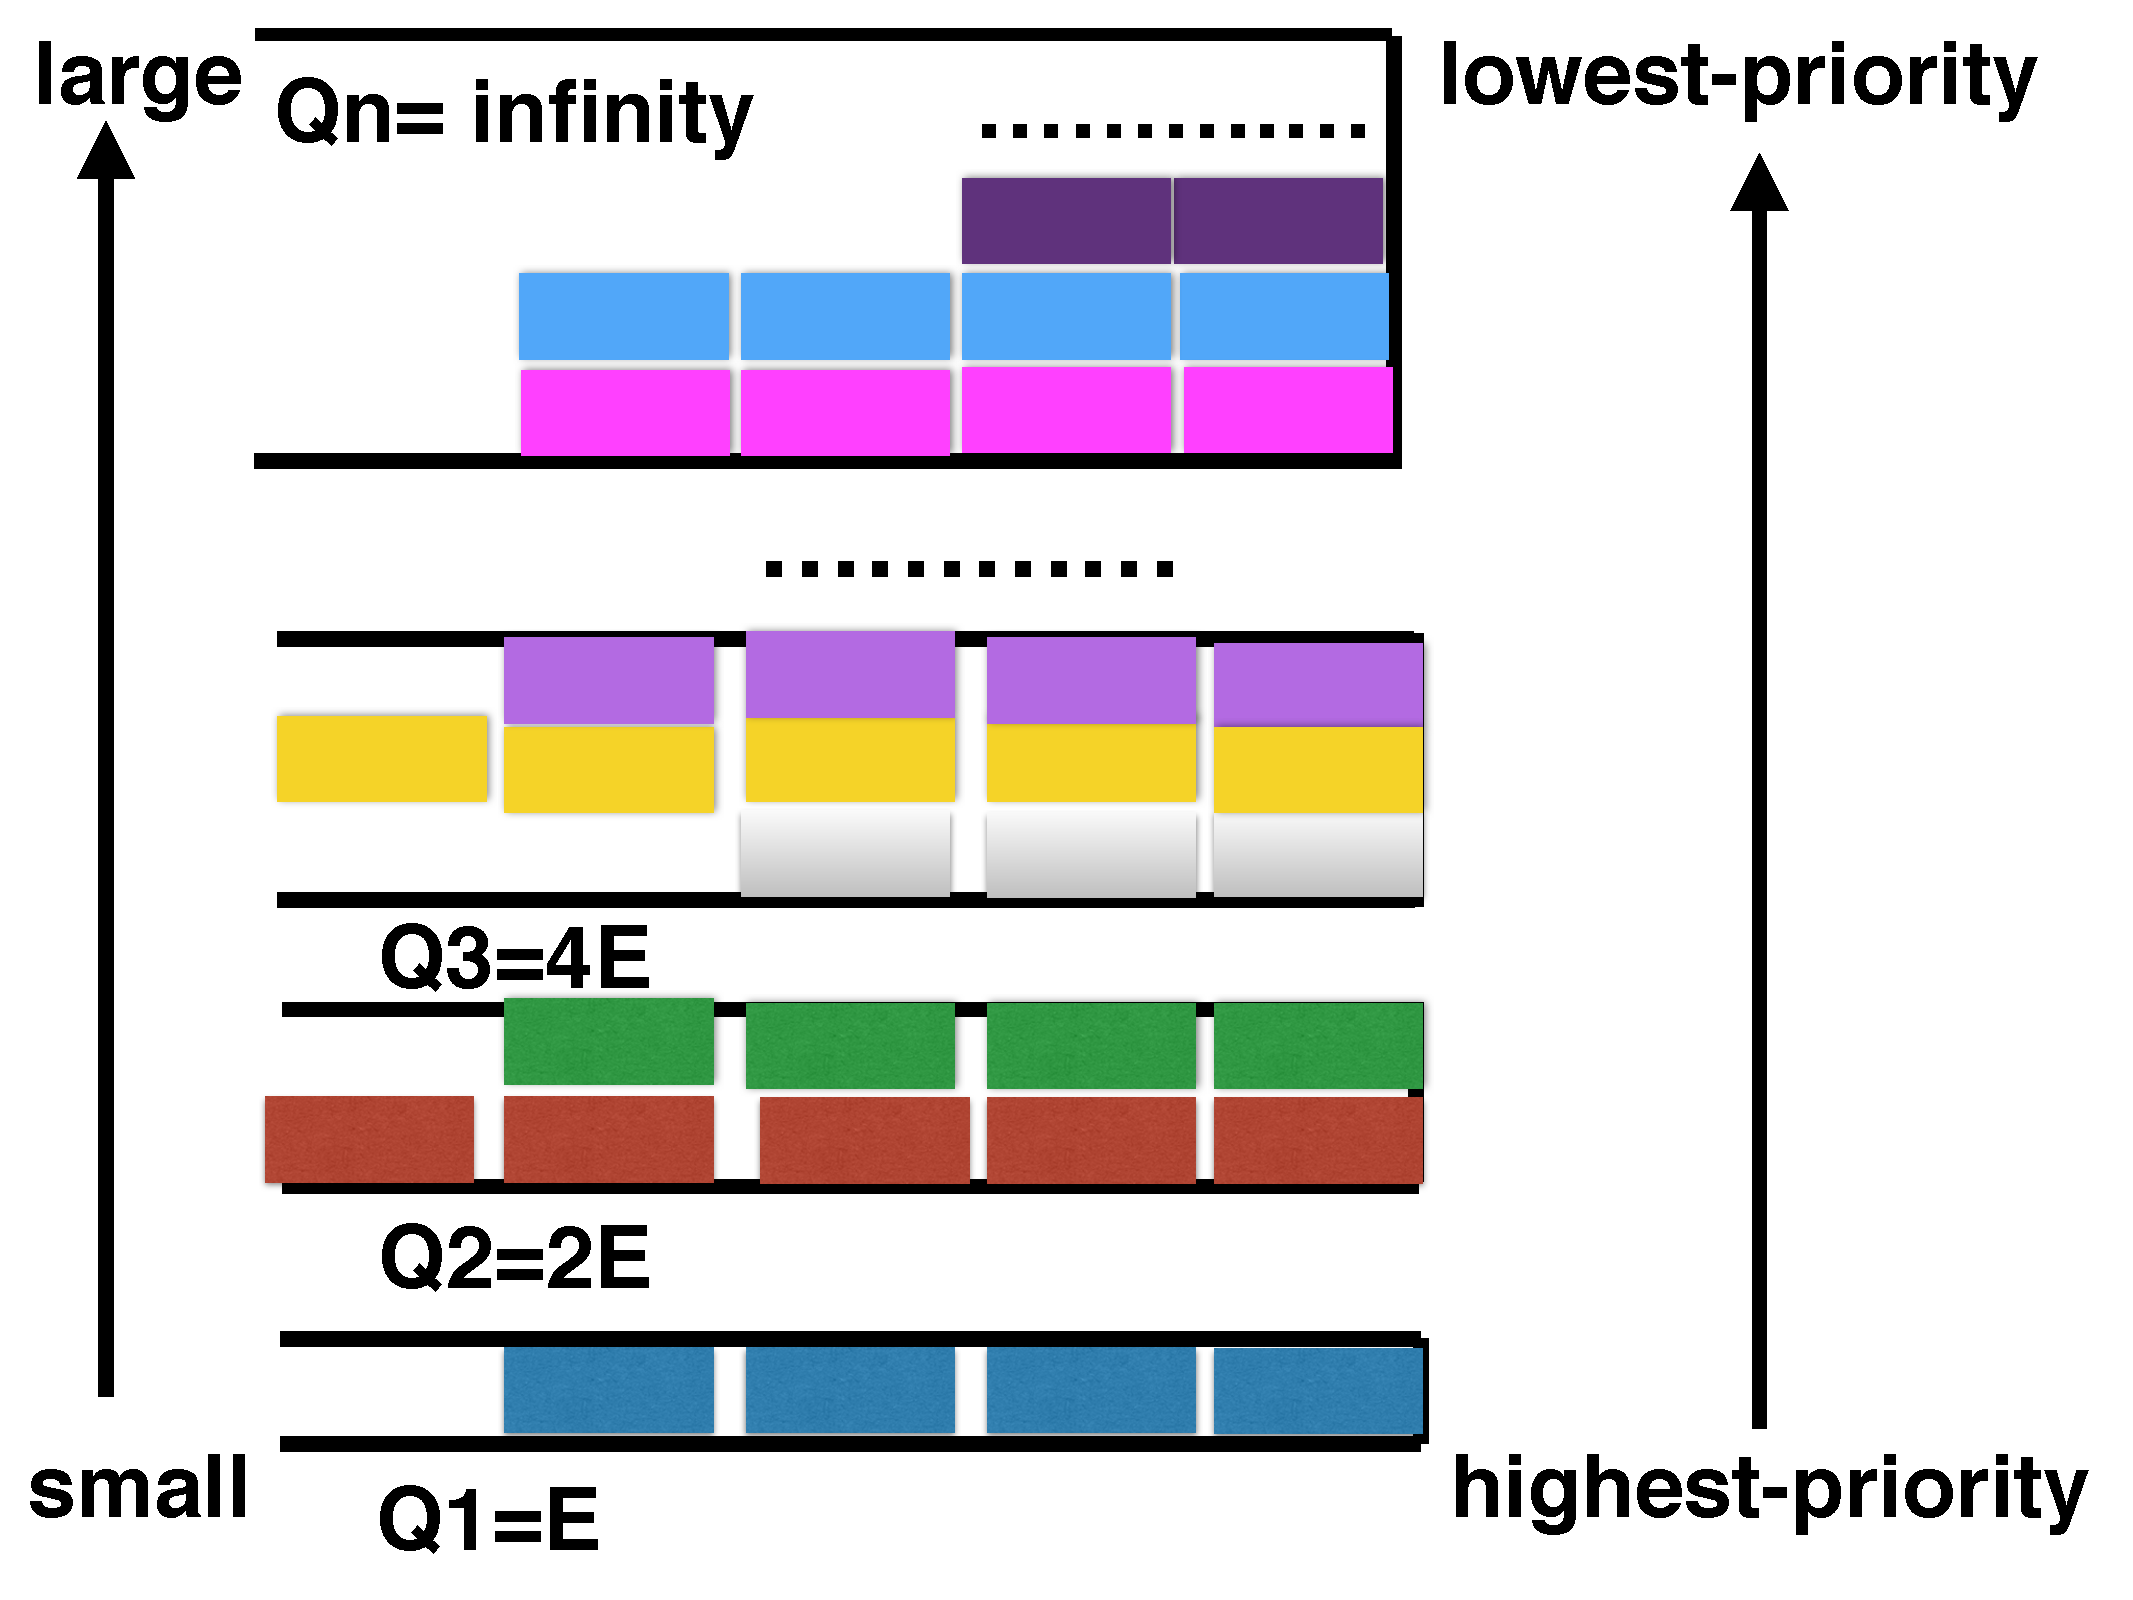
\includegraphics [width=0.8\columnwidth] {./figs/system/queue.pdf}
%\caption{Weight Priority Queue: from the bottom, the size of queue become larger and the priority lower }
%\label{queue-fig}
%\end{center}
%\end{figure}

%
%As the sequence of coflows is updated every T, however, in practice, some flows are always short and wait for T time may lead to bad performance.
%As a result, in our system, we set a threshold K,  flows whose size is smaller than K will get the lowest priority and this can avoid the condition of starvation.


\subsection{From offline to online}
The key of Algorithm \ref{offline} is to set the lowest priority to the coflow with the minimum weight-to-processing time ratio on the port with the maximum load,
and then handles the next-to-last coflow.
As today's data centers generally assign jobs with load balancing \cite{dean2008mapreduce}, 
so that we can make the relaxation of ignoring load difference of each port.
When a new coflow comes,  we can set the lowest priority to the coflow which has maximum per-port load. 
Then we get the online approach which is as Algorithm \ref{online-algorithm} shown.

\begin{algorithm} 
 \caption{Online approach to minimize average coflow weighted completion time}
 \begin{algorithmic}[1]\label{online-algorithm}
 \renewcommand{\algorithmicrequire}{\textbf{Input: }}
 \renewcommand{\algorithmicensure}{\textbf{Output:}}
 \REQUIRE Coflow set $\mathcal{C}$ ; active flow \emph{remaining} size $r_{i,j}^{(k)}$ from port i to port j, where $1 \leqslant i
 \leqslant m$,$1 \leqslant j \leqslant m$
 \ENSURE  $\gamma$
  \STATE $W\{1,2,...n\}\gets\{w_1,w_2,w_3...w_n\}$
  \STATE $L_i^{(k)}= \sum_{j=1}^mr_{i,j}^{(k)}$ for all k $\in$ $\mathcal{C}$ and i $\le$ m
   \STATE $L_{j+m}^{(k)}= \sum_{i=1}^mr_{i,j}^{(k)}$ for all k $\in$ $\mathcal{C}$ and j $\le$ m
    \STATE  $l^{(k)}$=$ \max \limits_{1 \le i \le 2m}L_i^{(k)}$ for all k $\in$$\mathcal{C}$ 
     \STATE  $\alpha^{(k)}$=W[k]/$l^{(k)}$ for all k $\in$ $\mathcal{C}$ 
     \STATE sort[$\alpha^{(1)}$,$\alpha^{(2)}$,$\alpha^{(3)}$...$\alpha^{(n)}$] in non-decreasing order and set the result to $\gamma$
     \end{algorithmic} 
 \end{algorithm}
 
 
 Algorithm \ref{online-algorithm} is called when a new coflow arrives. 
 Different from Algorithm \ref{offline}, Input of  Algorithm \ref{online-algorithm} is remaining flow size from each port pair.
 Line2$\sim$Line4 computes the load on each port. 
 Instead of considering load diversity on each port, we directly compute the ratio of weight and load at Line5.
At last, we sort the ratio of each coflow  in non-decreasing order. 
Comparing with the offline algorithm which has the O(n(m+n)) for-do loop, Algorithm  \ref{online-algorithm} only has sort operation at last. 
If we use insertion sorting, its main elementary operations is only O(m+nlogn) and this is much faster and easier than Algorithm \ref{offline}.

% Similar to \cite{chowdhury2014efficient}, the load of each coflow is:
%
%\begin{eqnarray} \label{weight_completion_gamma}
%g^{(k)}=\max(\max \limits_i \frac{ \sum_{j=1}^mf_{i,j}^{(k)}}{Rem(P_i^{(in)})},\max \limits_j \frac{ \sum_{i=1}^mf_{i,j}^{(k)}}{Rem(P_j^{(out)})})
%\end{eqnarray}

%$Rem(P_i^{(in)})$ denotes the remaining port capacity of ingress port $P_i^{(in)}$. $Rem(P_j^{(out)})$ denotes the remaining port capacity of egress port $P_j^{(out)}$. 
%In our assumption, the capacity of each port is 1. 

\subsection{Distance between the online and offline algorithm}
Compare with the offline algorithm, Algorithm \ref{online-algorithm} ignores load diversity and this may lead to performance loss.
In this section we study the performance gap between the online and the 2-approximate offline algorithm. 
Consider the schedule of 100 coflows served by a small-scale cluster consisting of 60 hosts. 
These hosts are connected with a non-blocking network fabric, where each port (both ingress and egress) has the capacity of 1 GB/s. 
Details of the simulator can be seen at Section \ref{evaluation}. 
Set coflows' arrival time to 0 and weight within 1 to 5.
Fig. \ref{online-offline-fig} shows the result. 

From Fig. \ref{online-offline-fig}, we can see the online algorithm performs close to the 2-approximate algorithms in total and only prolongs the transfer of large coflows. 
As coflows are generated randomly, we repeat the numerical simulation 200 times. 
Table \ref{tab:loss} shows the proportions of $\frac{avg \;wcct\  of \ online}{avg\; wcct \ of \  2-appr}-1$, where $avg\;wcct $ means average weighted coflow completion time.
We can see that 64\% cases have less than 0.025 of performance loss.
More than 91\% cases have the less than 0.1 performance gap and no cases have more than 0.15 performance loss.  

      \begin{table}[!htb]
          \centering
          \footnotesize
          \caption{Performance loss result} \label{tab:loss}
          \begin{tabulary}{\textwidth}{cccccr}
              \toprule
              $\leq 0\%$  & \multicolumn{1}{c}{$\leq 0.025$} & $\leq 0.05$& $\leq 0.1$ &$\leq 0.15$\\
              \midrule
              \multicolumn{1}{r}{0} & 64\%    &72\%    &91\%  &100\%  \\
             \bottomrule
          \end{tabulary}
      \end{table}
      
      
\begin{table}[!htb]
          \centering
          \footnotesize
          \caption{Comparison between the two algorithms} \label{tab:comparison}
          \begin{tabulary}{\textwidth}{ccccr}
              \toprule
              \#Scheme  & \multicolumn{1}{c}{Sched-Mode} & Procedure & Performance \\
              \midrule
              \multicolumn{1}{r}{2-appr} & offline    & Complex     & High \\
              \multicolumn{1}{r}{Yosemite} & online    & simple     & High \\
              \bottomrule
          \end{tabulary}
      \end{table}
      

As Table. \ref{tab:comparison} shown, we conclude comparing with the offline algorithm, online algorithm has little performance loss. 
Indeed, it is much more simple and can maintain relative high performance,
so that in reality, using the online algorithm to schedule coflow is a good choice.

\begin{figure}[b]
\begin{center}
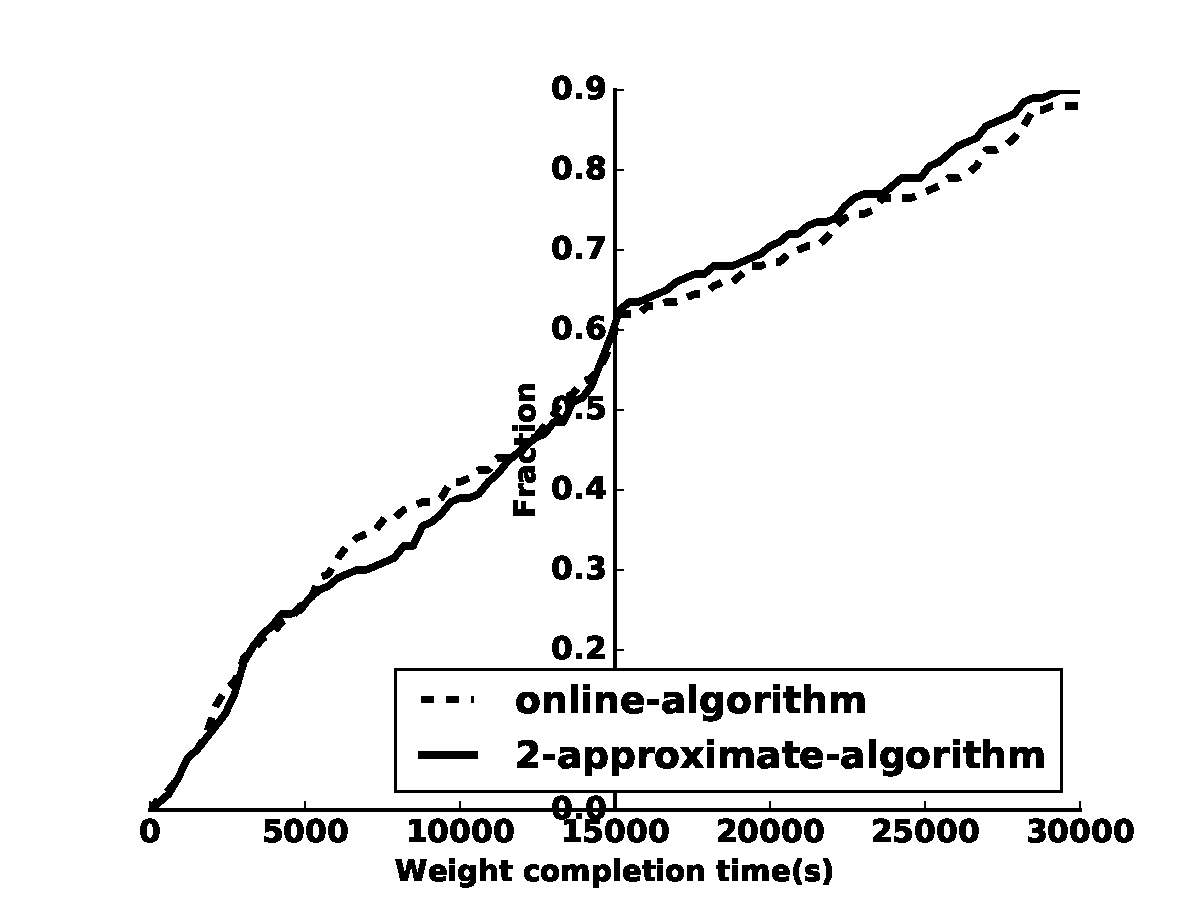
\includegraphics [width=0.8\columnwidth] {./figs/performance/online_offline.pdf}
\caption{[Simulation] Performance comparison between 2-approximate algorithm and online algorithm}
\label{online-offline-fig}
\end{center}
\end{figure}


\section{Yosemite System}\label{Yosemite system}

In this section, we introduce the design of Yosemite which is a system aims to minimize average weighted coflow completion time. 
Yosemite includes about 6000 lines  of scala code and is similar to Alluxio\cite{alluxio}, hadoop\cite{hadoop} whose designs follow the actor model\cite{actor}.
 Yosemite uses Akka \cite{Akka} for message transferring and kryo \cite{kryo} for object serialization. 
 Code of Yosemite can be downloaded at \cite{Yosemite}.
 In this section, we first introduce actors of Yosemite and the communication between them.
 Then we introduce the usage of Yosemite.
  \begin{figure}[b]
\begin{center}
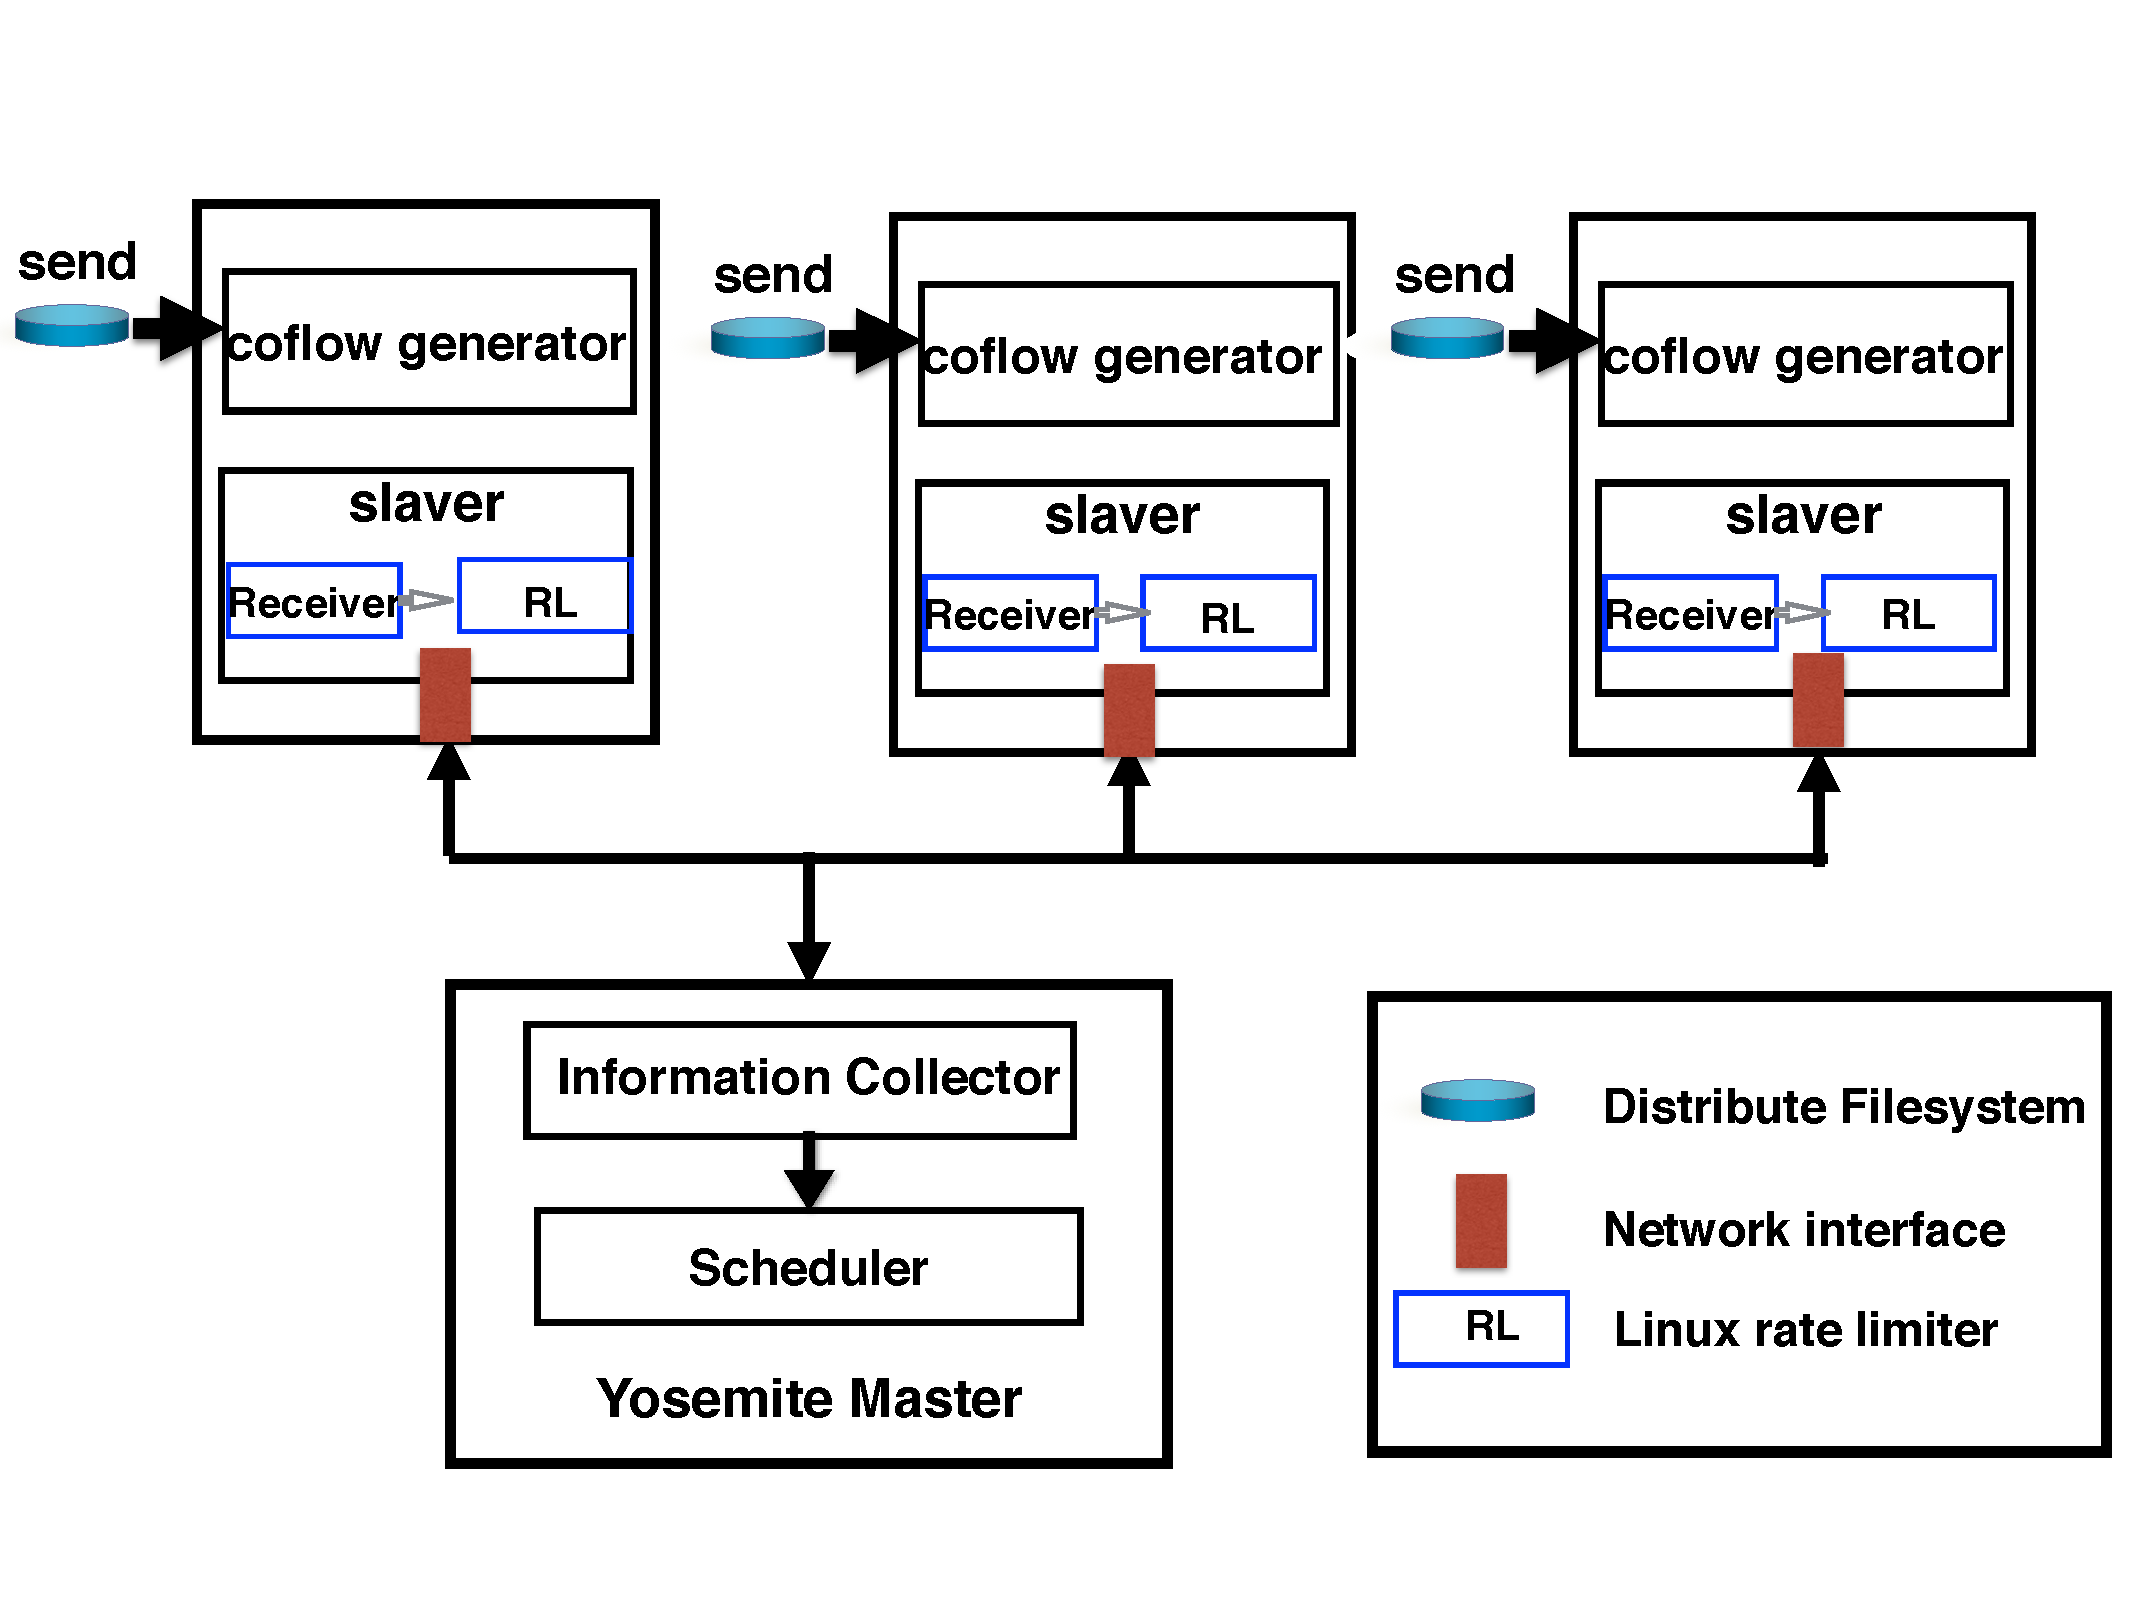
\includegraphics [width=0.8\columnwidth] {./figs/background/system.pdf}
\caption{Yosemite architecture. Computation frameworks interact with Yosemite through a client library}
\label{System-design-fig}
\end{center}
\end{figure}

\subsection{Actors and communication}  
\begin{algorithm} 
\caption{Procedure of bandwidth allocate}
\begin{algorithmic}[1]\label{bandwidth_allocate}
\renewcommand{\algorithmicrequire}{\textbf{Input: }}
\renewcommand{\algorithmicensure}{\textbf{Output:}}
\REQUIRE Sorted coflow set $\gamma$, Remaining capacity for ports set $Rem(.)$
\ENSURE  bandwidth of each coflow, Remaing capacity for ports set $Rem(.)$
\FOR{k $\in \gamma$ }
 \STATE Compute Load $g^{(k)}$ according to (\ref{weight_completion_gamma})
 \FOR{$f_{i,j}$$ \in k$ }
 \STATE $b_{i,j}=f_{i,j}/g^{(k)}$
\STATE $Rem(P_i^{(in)})-=b_{i,j}$
\STATE $Rem(P_j^{(out)})-=b_{i,j}$
 \ENDFOR
\ENDFOR
\end{algorithmic} 
\end{algorithm}


\begin{algorithm} \label{procedure_master}
\caption{Procedure of the master}
\begin{algorithmic}[1]\label{scheduler}
\renewcommand{\algorithmicrequire}{\textbf{Input: }}
\renewcommand{\algorithmicensure}{\textbf{Output:}}
\REQUIRE Coflow F
\ENSURE  bandwidth of each flow 
\STATE $\mathcal{C}=\mathcal{C}\cup F $
\STATE Sort $\mathcal{C}$ according to Algorithm \ref{online-algorithm}
\STATE Allocate bandwidth to $\mathcal{C}$ according to Algorithm \ref{bandwidth_allocate}
\STATE Distribute unused bandwidth to $\mathcal{C}$ for all ports
\STATE Send $b_{i,j}$ to corresponding Slave
\end{algorithmic} 
\end{algorithm}

Fig. \ref{System-design-fig} shows the architecture of Yosemite.
There are two type of nodes: master and worker. 
Each worker node includes two main components: Client and Slave.
Client contains API Daemon and Rate Limiter. 
API Daemon is used to interact with applications and Rate Limiter is responsible for throttling flow rate according to the computation results sent from master.
Slave has two long running server: data server and comm server. 
Comm server communicates with master and data server is used to send data.
Master node is the brain of the system.
It collects coflow information from worker and sends bandwidth information to worker. 
It also has two components: slave and scheduler.
The function of slave is same as that as worker node.
Yosemite Scheduler performs coflow sorting and bandwidth computation.
Algorithm \ref{scheduler} shows the operation detail of scheduler.

 
Algorithm \ref{scheduler} is called when a new coflow arrives. Line1$\sim$Line2 tries to sort coflow.  
It calls the online coflow  scheduling Algorithm \ref{online-algorithm}. 
Line3  tries to allocate bandwidth to coflow on the basis of sequence that is computed at Line2. 
Algorithm \ref{bandwidth_allocate} has two key steps. 
Firstly, it computes the bottleneck time of each coflow.
The computation method of it is: 
\begin{eqnarray} \label{weight_completion_gamma}
g^{(k)}=\max(\max \limits_i \frac{ \sum_{j=1}^mf_{i,j}^{(k)}}{Rem(P_i^{(in)})},\max \limits_j \frac{ \sum_{i=1}^mf_{i,j}^{(k)}}{Rem(P_j^{(out)})})
\end{eqnarray}
Where Rem(.) denotes the remaining bandwidth of an ingress or egress port estimated by the scheduler.
(\ref{weight_completion_gamma}) computes out transfer time of the slowest flows that belongs to coflow $F^{(k)}$.
After this, on the basis of bottleneck time, it computes bandwidth $b_{i,j}$ for each flow that transfers from port i to port j 
Then master updates port available bandwidth as Line5$\sim$Line6 shown.  
After the process of Algorithm.\ref{bandwidth_allocate}, scheduler calculates out bandwidth for each flow.
At last, scheduler sends the result to each worker, then worker sends flows according to the computation result.

In particular, communication between components is important for a correct distributed, concurrent, fault-tolerant and scalable application.
As messages transferring between components needs timely responds, keeping responsive in the face of failure, staying responsive under varying workload. 
In Yosemite, Comm Server is responsible for this. 
Comm Server extends Akka \cite{Akka}. 
Using the library provided by Akka, Comm Server can provide stable communication for Yosemite components. 

\subsection{Work-conserving allocation}
Line4 of Algorithm \ref{scheduler} aims to provide work conserving allocation for resources.
Just using the computation result of Algorithm \ref{bandwidth_allocate}, extra network resources may be wasted.
To prevent this happening, we allocate the remaining bandwidth fair to the corresponding flows that transfer from the port.
 With work-conserving allocation, resources can be used more efficiency, so that less resources will be wasted.

\subsection{Fault-tolerance}
Master is the "brain" of Yosemite. 
It collects information from slave and computes the bandwidth of each flow. 
However, for some extreme cases,  master may be crushed. 
If this happened, the system can not work any more. 
Although Akka provides fault-tolerant strategy which will restart scheduler when it crush down, scheduling information will be lost.
To prevent this happen, we start a monitor which stores the real-time state of master.    
When master collapses, the monitor tries to restart  the master and lets it resume the state just the same as no-crushing down. 
Also, work node may also crash. 
If this happens, master will try to restart the worker node daemon to let it work normally.

\subsection{API}
Yosemite provides API like DOT \cite{tolia2006architecture} and Varys \cite{chowdhury2014efficient} to abstract the underlying scheduling and communication mechanisms. 
User jobs do not require any modifications, but should create Yosemite client to interact with the master. 
The client of Yosemite provides 4 key API just as Table. \ref{tab:API} shown.

\begin{table}[!htb]
          \centering
          \footnotesize
          \caption{Yosemite API} \label{tab:API}
          \begin{tabulary}{\textwidth}{ccccr}
              \toprule
              Name  & \multicolumn{1}{c}{parameters} & Return & Description \\
              \midrule
              \multicolumn{1}{r}{RegisterCoflow} & coflowdesc,weight    & coflowId     & Regisger a coflow \\
              \multicolumn{1}{r}{Send} & coflowId,size,dst    & bool     & Send size data to dst \\
              \multicolumn{1}{r}{Receive} & coflowId    & bool     & Receive a flow \\
              \multicolumn{1}{r}{ReleaseCoflow} & coflowId,   & bool     & Release coflow \\
              \bottomrule
          \end{tabulary}
      \end{table}
      
     
Register takes coflow description and weight of the coflow as parameters.
After sending the register information to master, coflow id will be returned to worker node.
Send tasks coflowId and IP address of destination node as parameters.
This method sends a flow that belongs to coflowId.
 Receive tasks coflowId as the parameter.
 This method is used to receive data belongs to the corresponding coflow.
 If return true, denoting worker receivers data successfully. 
 Otherwise it will return false.
ReleaseCoflow takes coflowId as the parameter and it is used to release the coflow when all flows belong to the coflow finish transferring.



\section{evaluation} \label{evaluation}
\begin{figure}[b]
\begin{center}
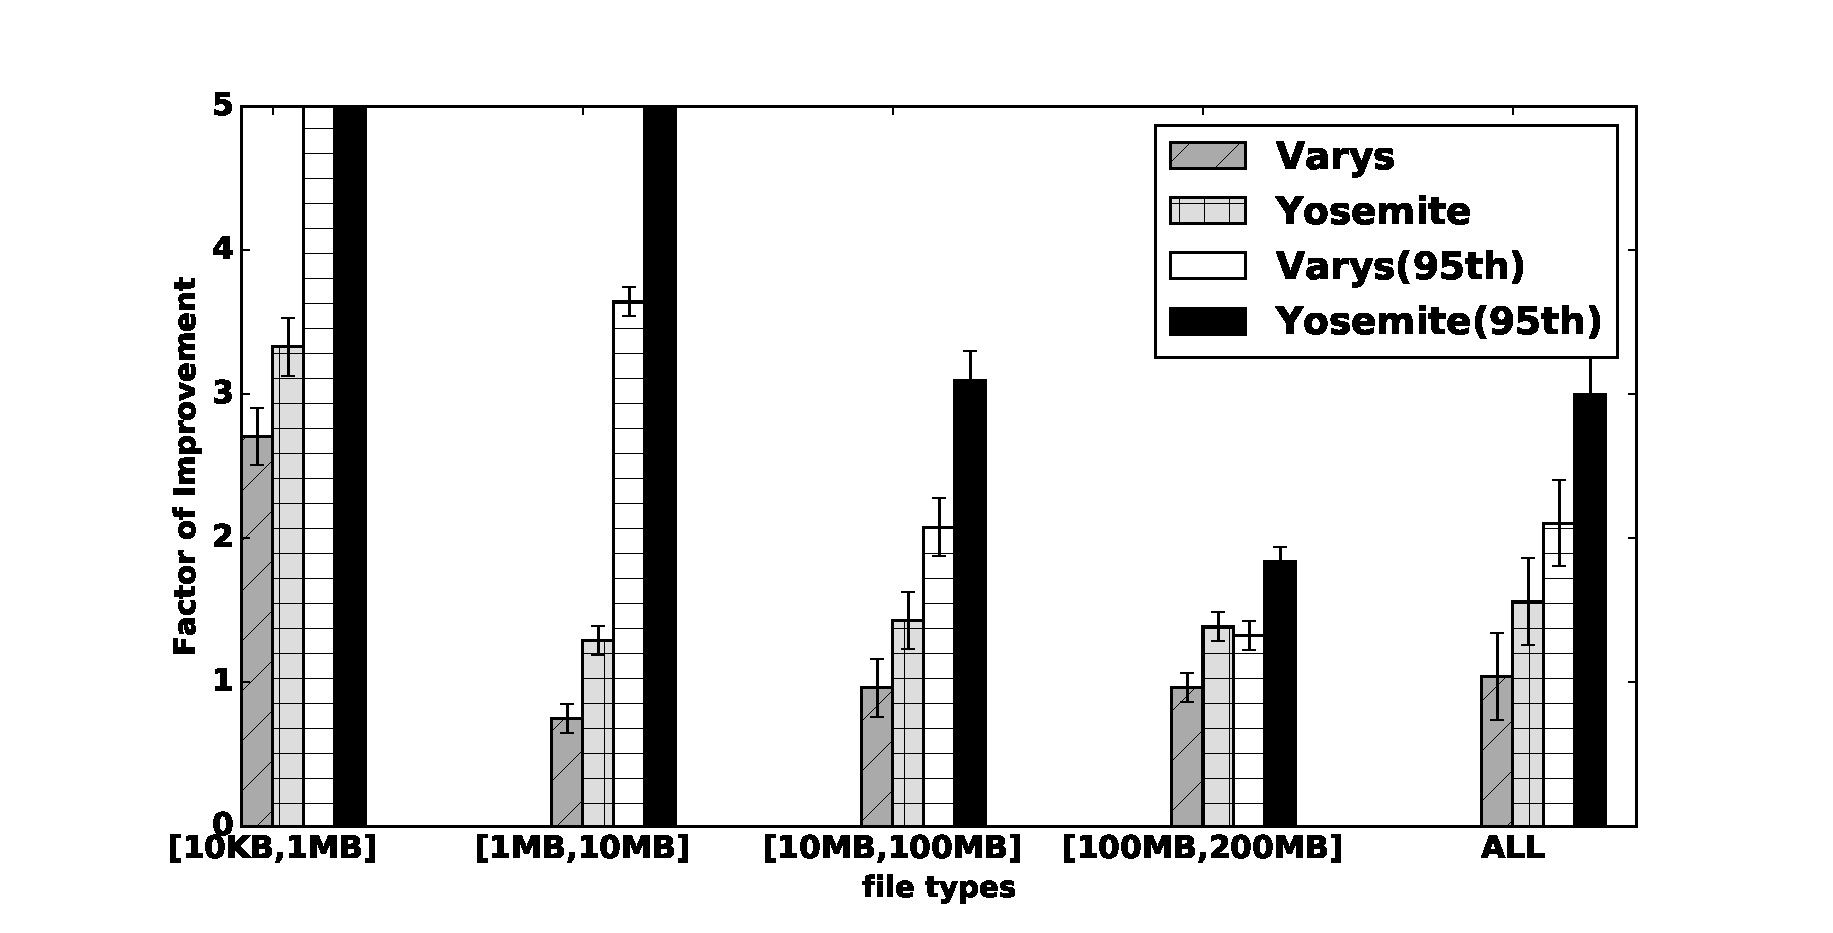
\includegraphics [width=1.0\columnwidth] {./figs/fake/fake2.eps}
\caption{[Cloud] File distribute application performance}
\label{distribute-fig}
\end{center}
\end{figure}

We evaluate Yosemite at our openstack \cite{openstack} platform.
Our private cloud can run at most 80 virtual machines (2 Cores, 4GB Mem) simultaneously. 
To evaluate a slightly larger scale experiments, some VMs will start at most 3 dockers.
For larger scale experiments, we use trace-driven simulation. 
Main results of our evaluation are as follows:

\begin{itemize}[\IEEEsetlabelwidth{Z}]

\item  Running file distribute application at our private cloud platform, we find Yosemite achieves 30\% average improvement against Varys.

\item Using facebook trace\cite{chowdhury2014efficient} with randomly generating weight, 
Yosemite improves about $30\%$, $40\%$, $50\%$ over Varys \cite{chowdhury2014efficient}, Aalo \cite{chowdhury2015efficient} and Barrat \cite{dogar2014decentralized} on reducing average coflow weighted completion time respectively.
However,  comparing with Varys, it only has $5\%$ performance gap on reducing average coflow completion time.

\item Under different length, width, weight and concurrent number of coflows, 
we find Yosemite improves more under larger length variance, width variance, weight variance and concurrency.

\item Comparing with the LP-based algorithm \cite{qiu2015minimizing} , Yosemite has only less than $10\%$ performance loss. 

\end{itemize}

\subsection{methlogy}

\textbf{Experiment settings}. 
In some of our experiment we use the traffic of Facebook that was collected from a 3000-machine cluster with 150 racks \cite{chowdhury2014efficient}. 
As the original trace does not contain information of weight settings, we randomly generate weight within 1 to 10.  
The original cluster had a 10 : 1 core-to-rack oversubscription ratio with a total bisection bandwidth of 300 Gbps.
 Due to hardware limits, in our testbed experiment, we limit the bandwidth of ingress and egress port capacity to 1Gbps and maintain the characters of the original traffic. 
In our experiment, coflows are categorized to be four types in terms of their length (the size of the largest flow in bytes for a coflow) and width (the number of parallel flows in a coflow): Narrow\&Short(N-S), Narrow\&Long(N-L), Wide\&Short(W-S), and Wide\&Long(W-L), where a coflow is considered to be short if its length is less than 100 MB, and narrow if it involves at most 20 flows.

\textbf{Metrics}. In our experiment,  metrics for comparison is the improvement in average weighted coflow completion time of jobs (when its last task finished) in the workload. 
In this paper, we use factor of improvement as our metrics. The definition of factor of improvement of current method is :

\begin{eqnarray} \label{improvement}
Factor \;of\; improvement=\frac{baseline\; avg \;WCCT}{current\;avg \;WCCT}
\end{eqnarray}
Note, in this paper, we use TCP-fair sharing as the default baseline method.
\begin{figure}[b]
\begin{center}
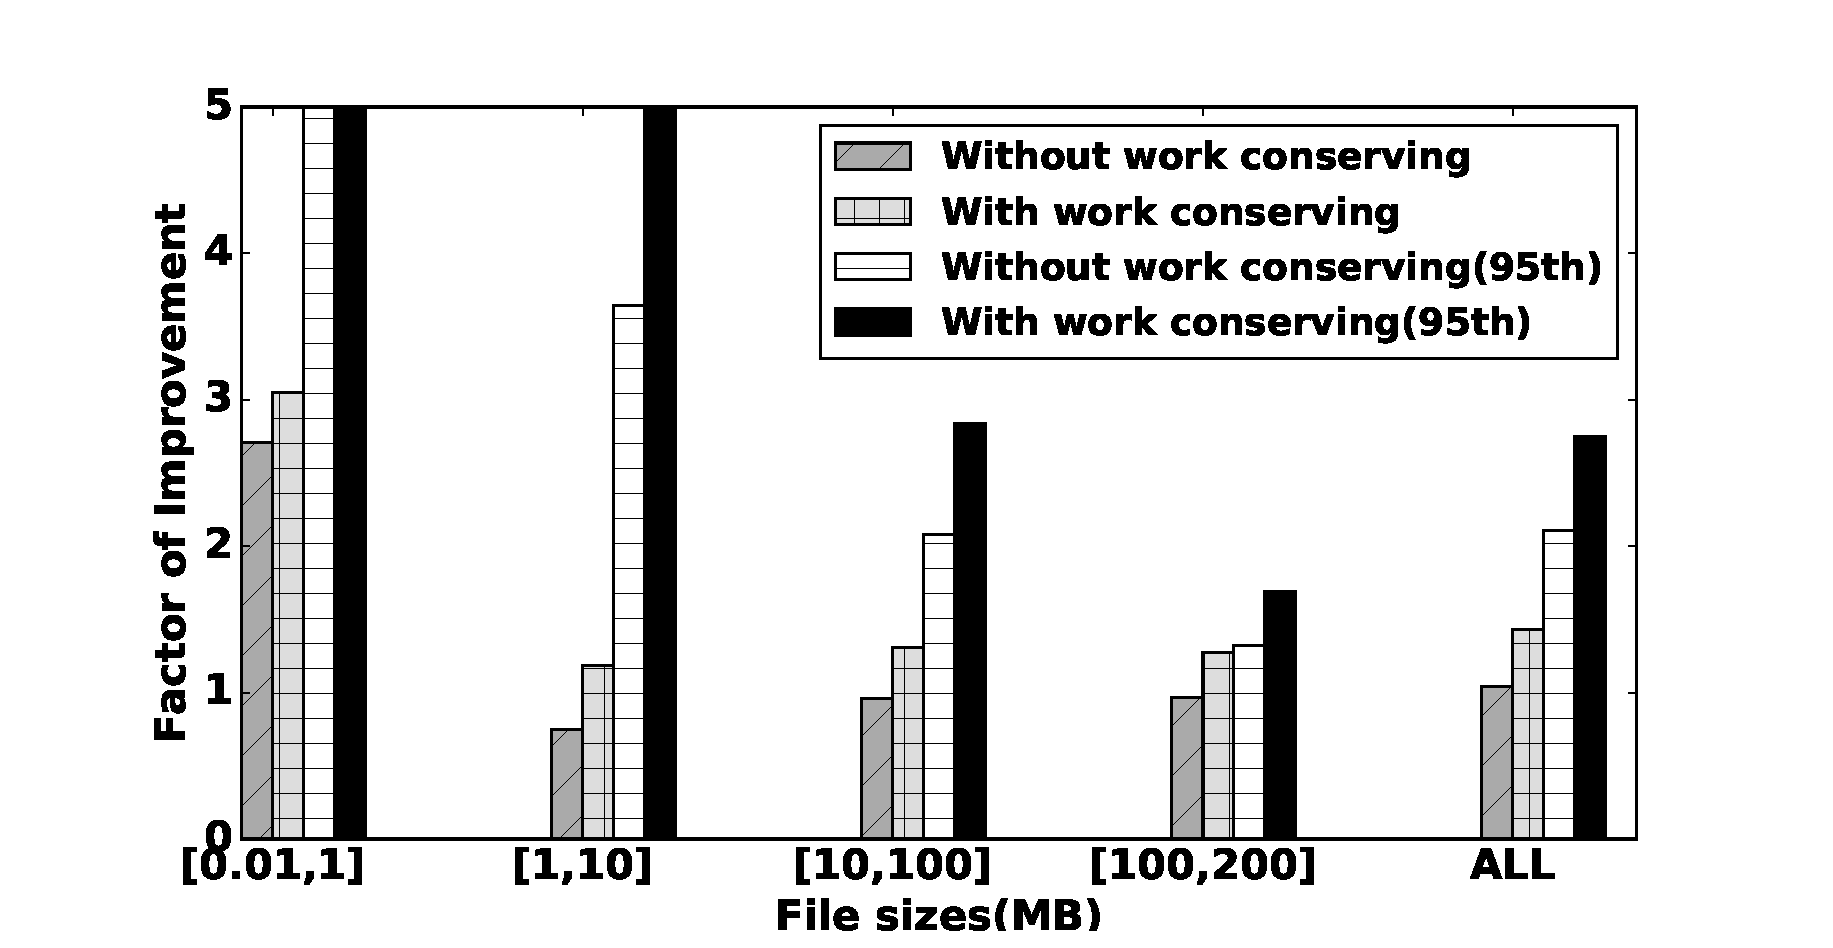
\includegraphics [width=1.0\columnwidth] {./figs/fake/fake4.eps}
\caption{[Cloud] With and without work conserving}
\label{conserving-fig}
\end{center}
\end{figure}
 \begin{figure}[!t]
\centering
\subfigure[Computation time of scheduler] {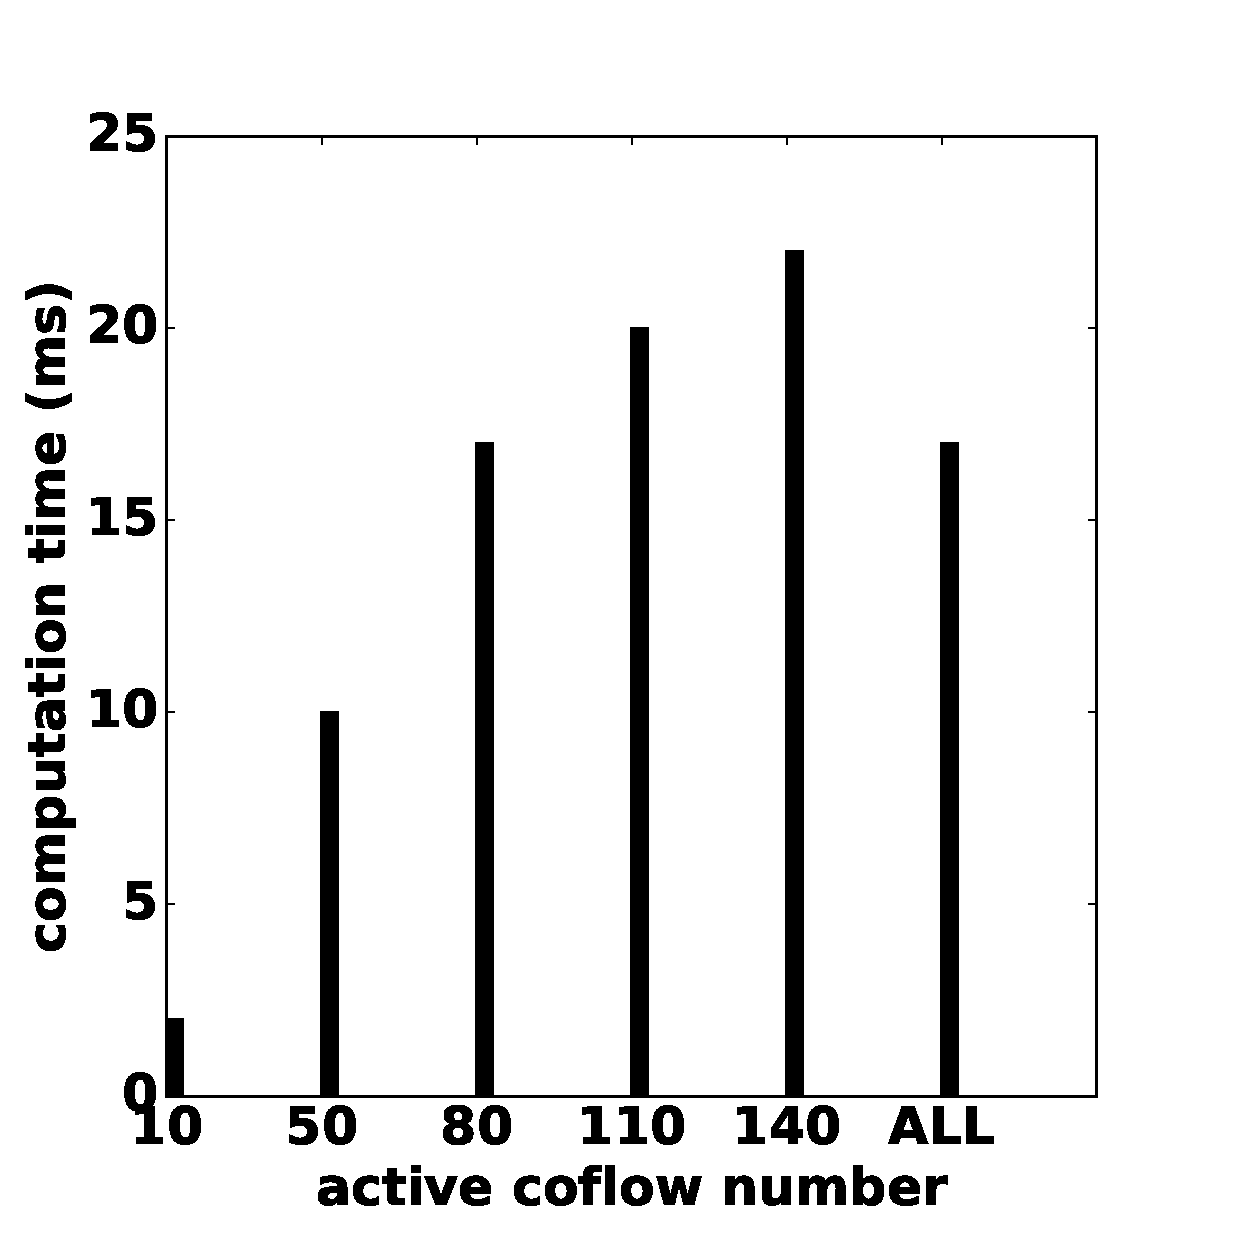
\includegraphics[width=1.6 in]{./figs/fake/fake5.eps}}
\hspace{0.1in}
\subfigure[Error messages frequency] {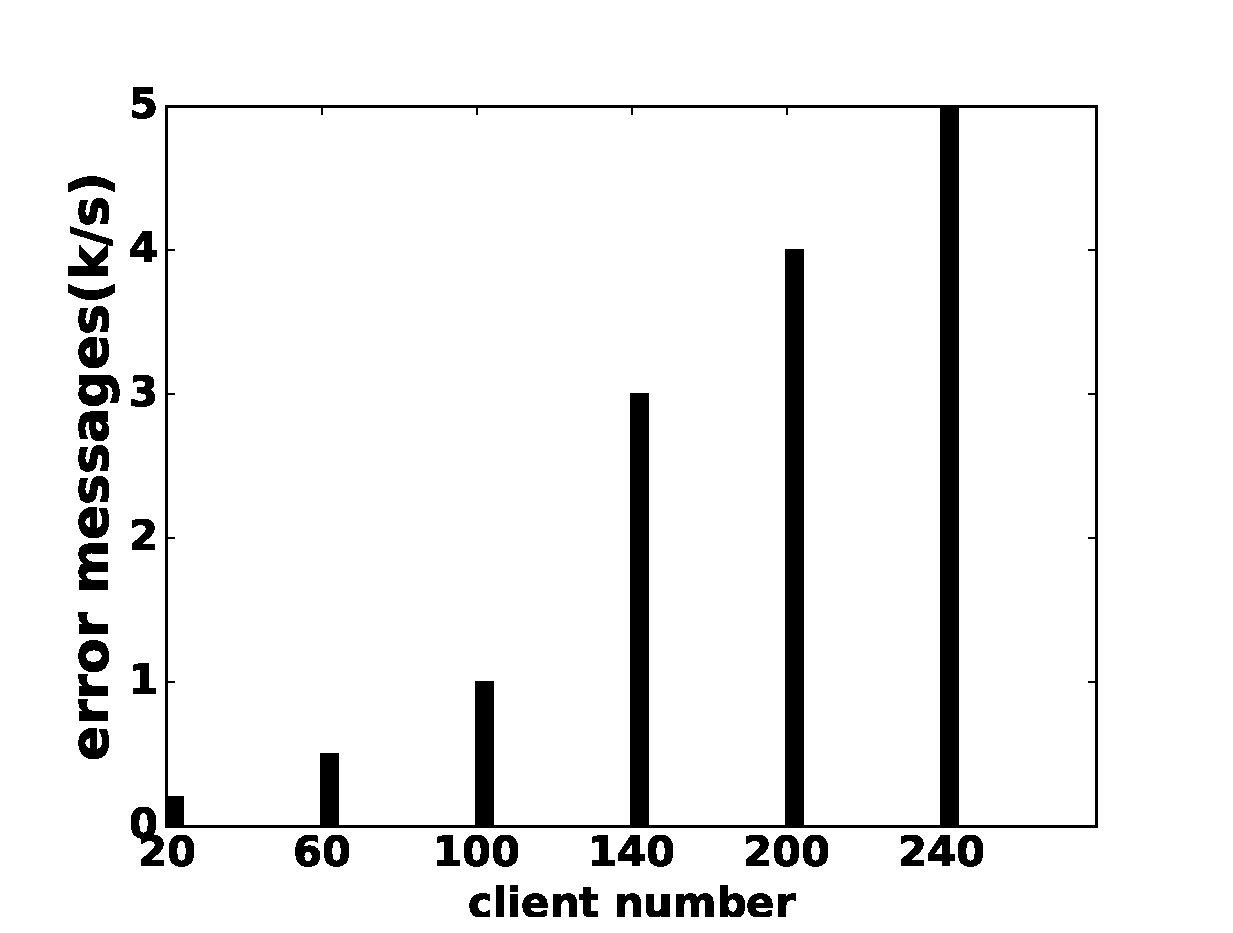
\includegraphics[width=1.6 in]{./figs/fake/fake6.eps}}
\hspace{0.1in}
\caption{[Cloud] Overheads of Yosemite}
\label{overheads_fig}
\vspace{-0.1 in}
\end{figure}
\begin{figure}[b]
\begin{center}
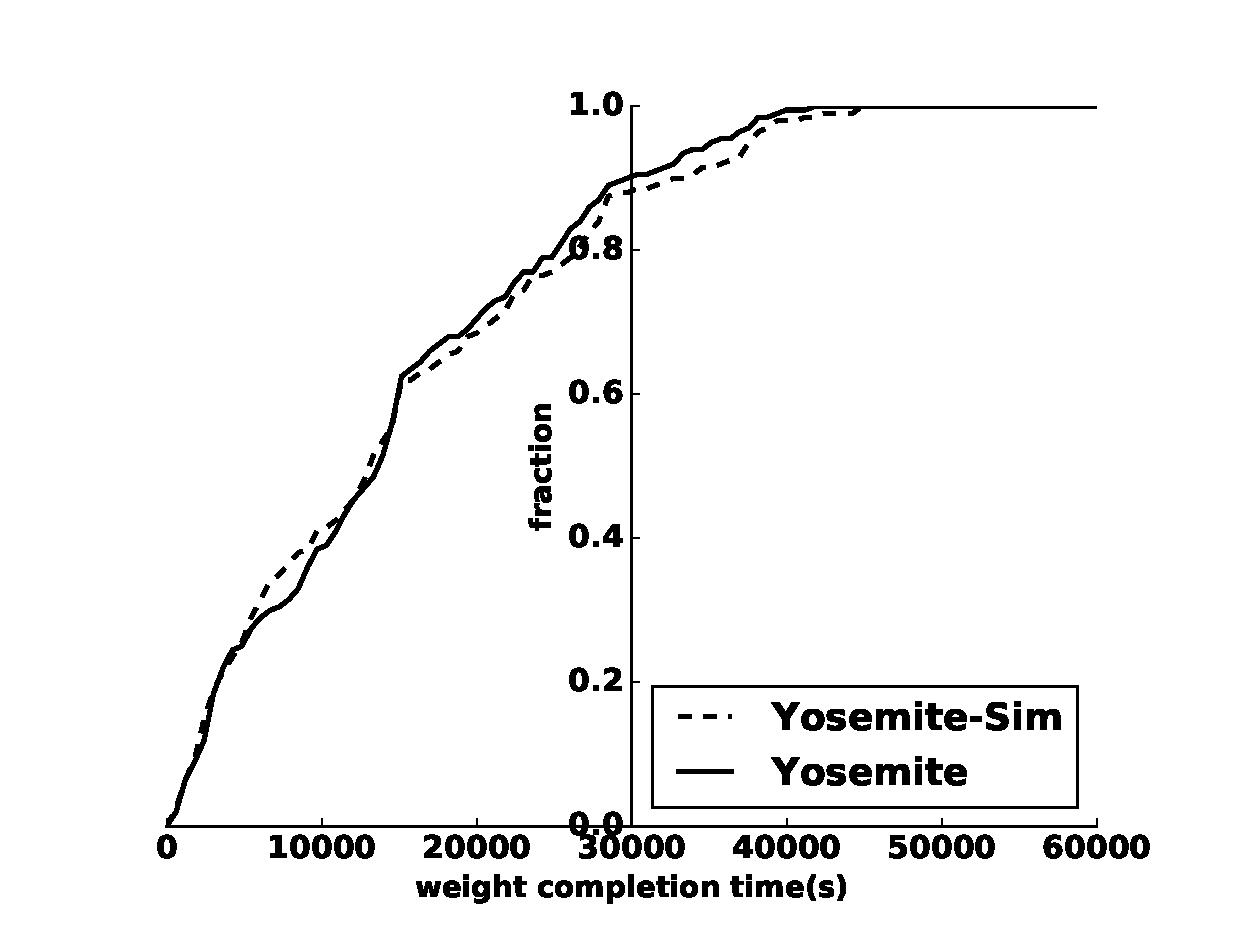
\includegraphics [width=0.8\columnwidth] {./figs/fake/fake3.eps}
\caption{[Cloud] Performance comparison between Yosemite and Yosemite-sim under the same settings}
\label{sim-real}
\end{center}
\end{figure}

\begin{figure*}[!t]
\centering
\subfigure[Improvement of WCCT] {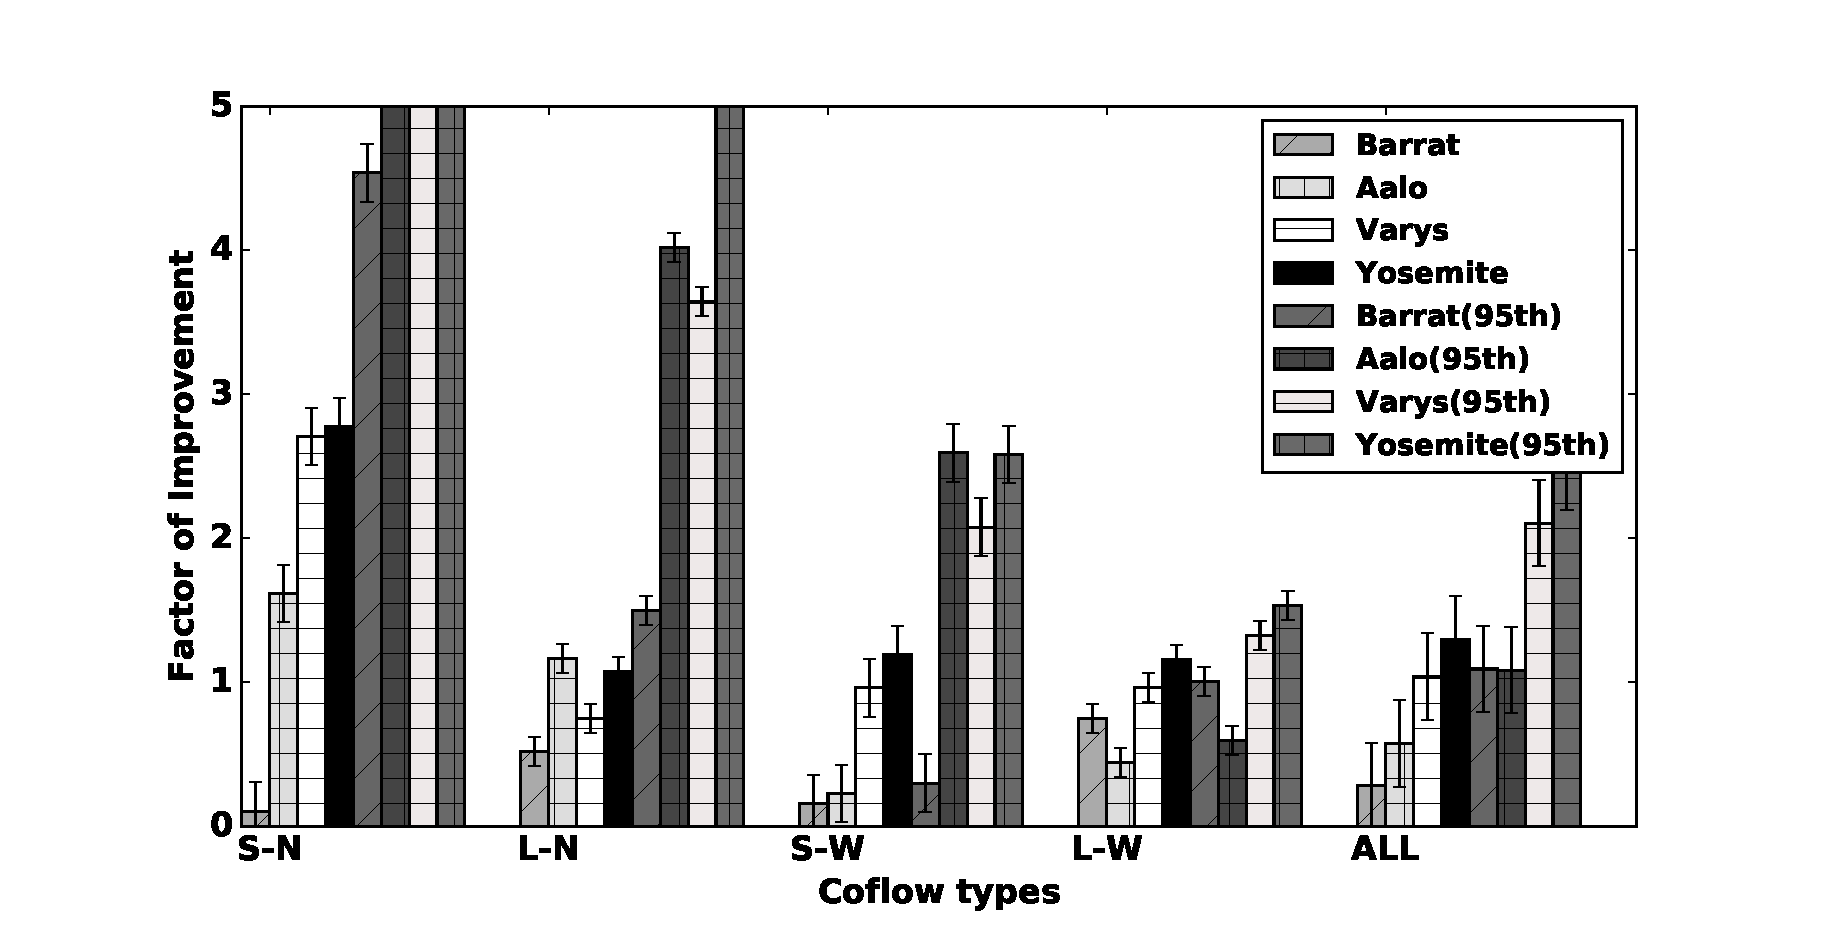
\includegraphics[width=4.9 in]{./figs/real/weight_real_type.eps}}
\hspace{0.1in}
\subfigure[Distribution of WCCT(s)] {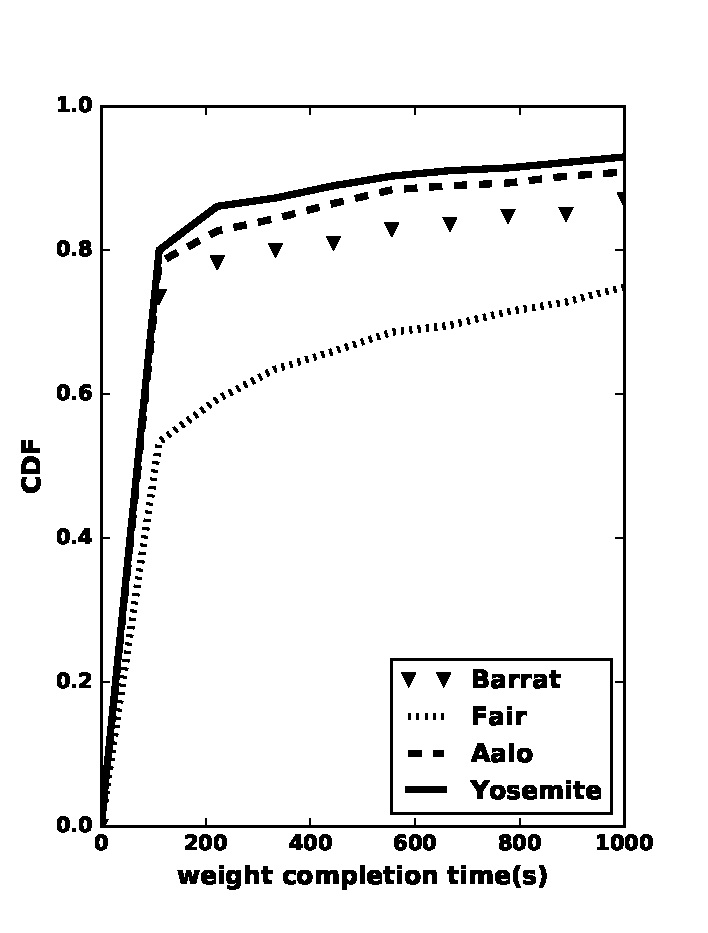
\includegraphics[width=2.05 in]{./figs/real/weight_CDF_compare.eps}}
\caption{[Simulation] Detail of WCCT for Yosemite, Barrat, Varys,  Aalo, TCP fair-sharing under real data center traffic trace}
\vspace{-0.1 in}
\label{evalution_real_weight_fig}
\vspace{-0.1 in}
\end{figure*}



\begin{figure*}[!t]
\centering
\subfigure[Improvement of CCT] {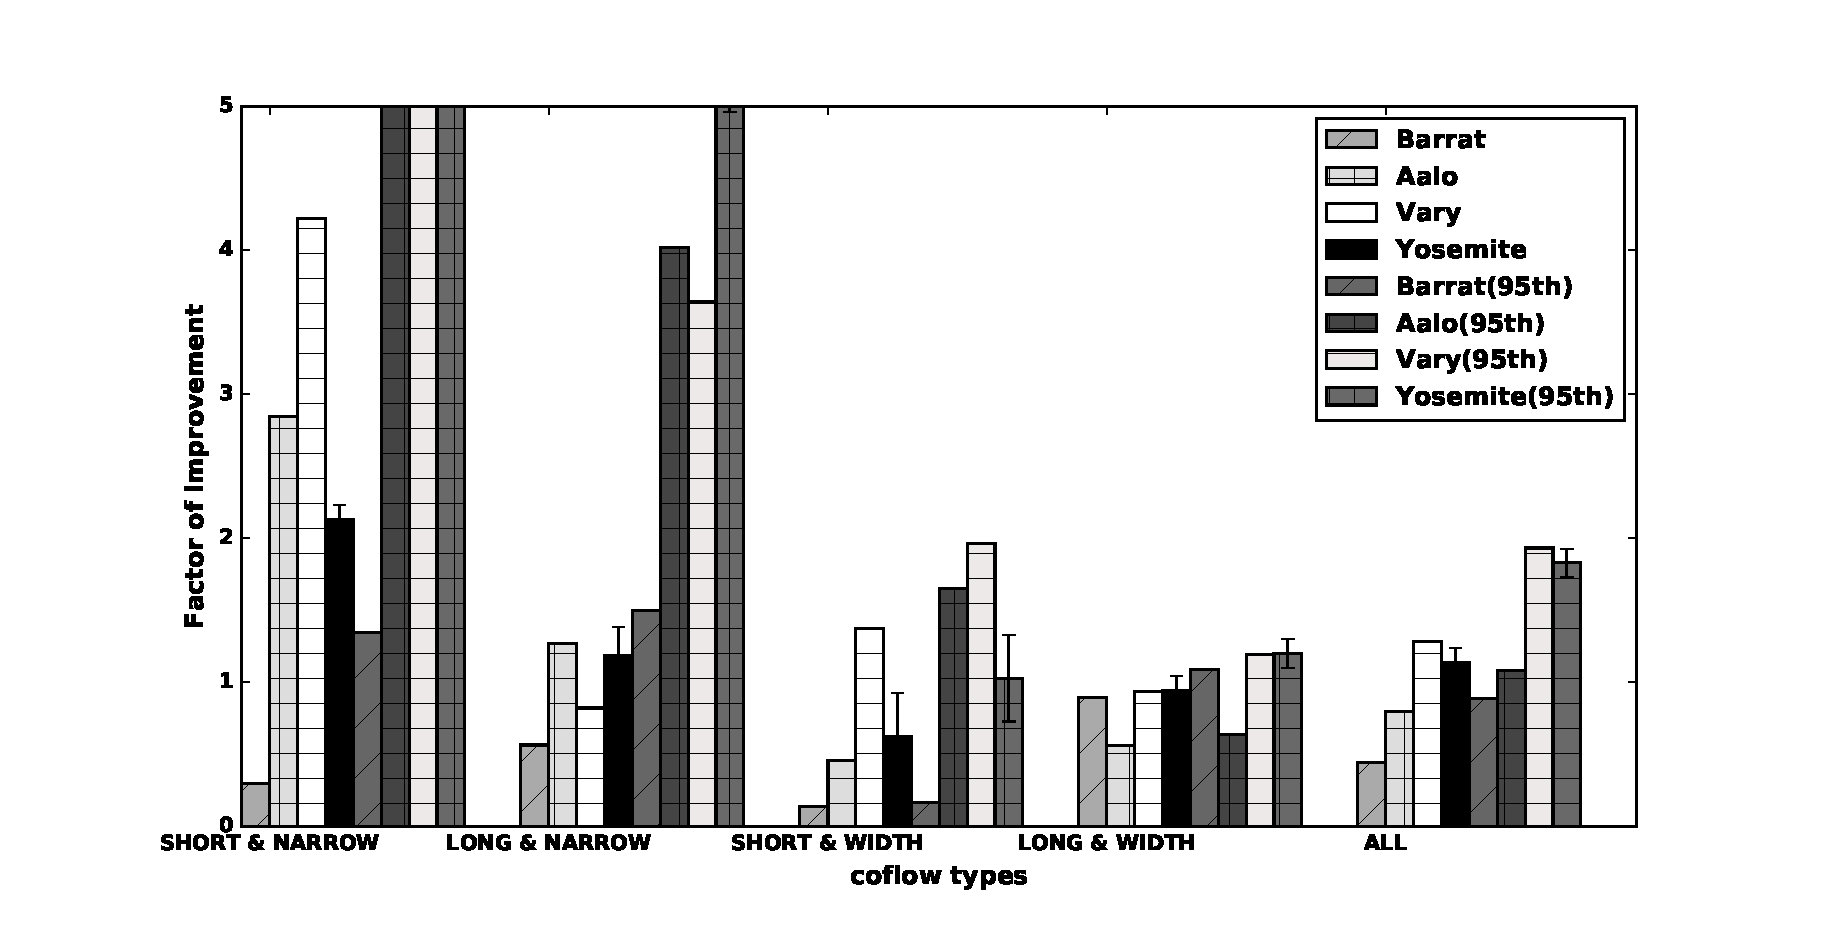
\includegraphics[width=4.9 in]{./figs/completion/real_type.eps}}
\subfigure[Distribution of CCT(s)] {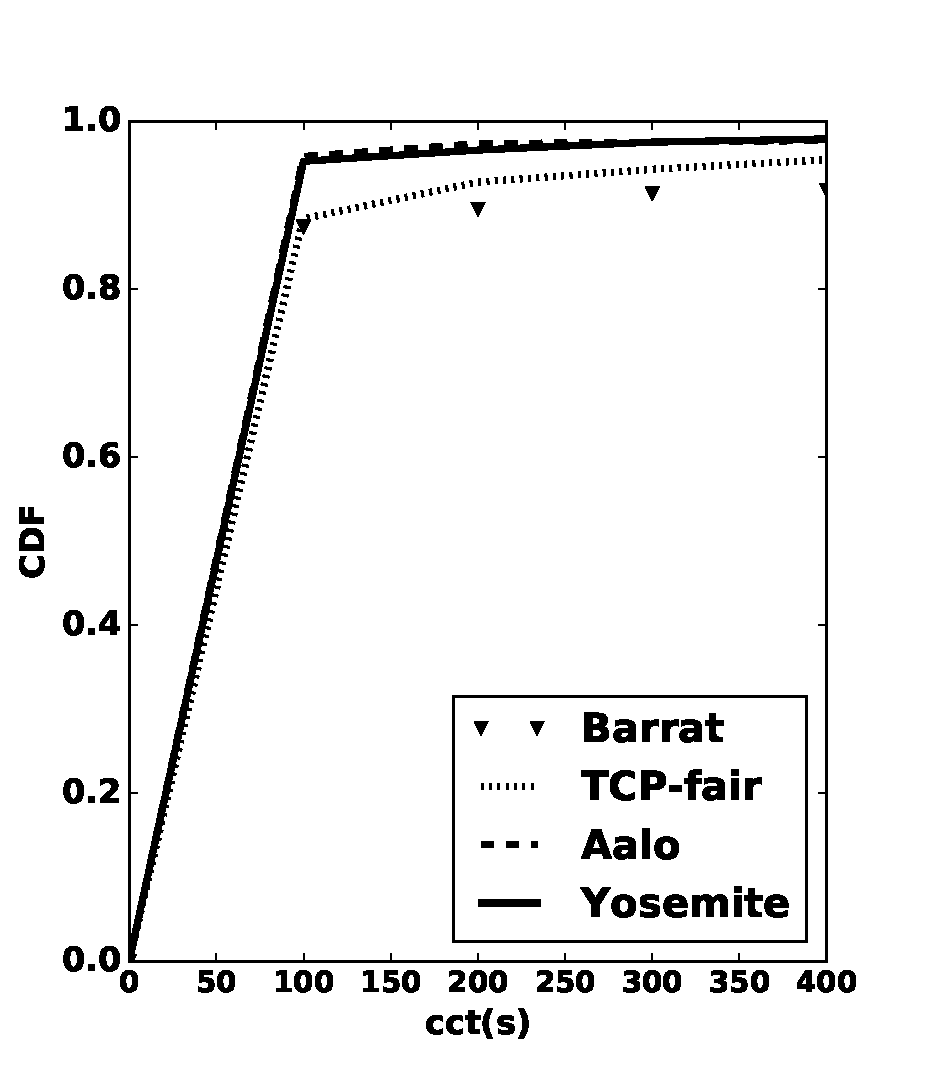
\includegraphics[width=2.1 in]{./figs/completion/CDF_compare.eps}}
\caption{[Simulation] Detail of CCT for Yosemite, Barrat, Varys,  Aalo, TCP fair-sharing under real data center traffic trace.}
\label{evalution_real_fig}
\end{figure*}

 \begin{figure*}[!t]
\centering
\subfigure[Impact of coflow length] {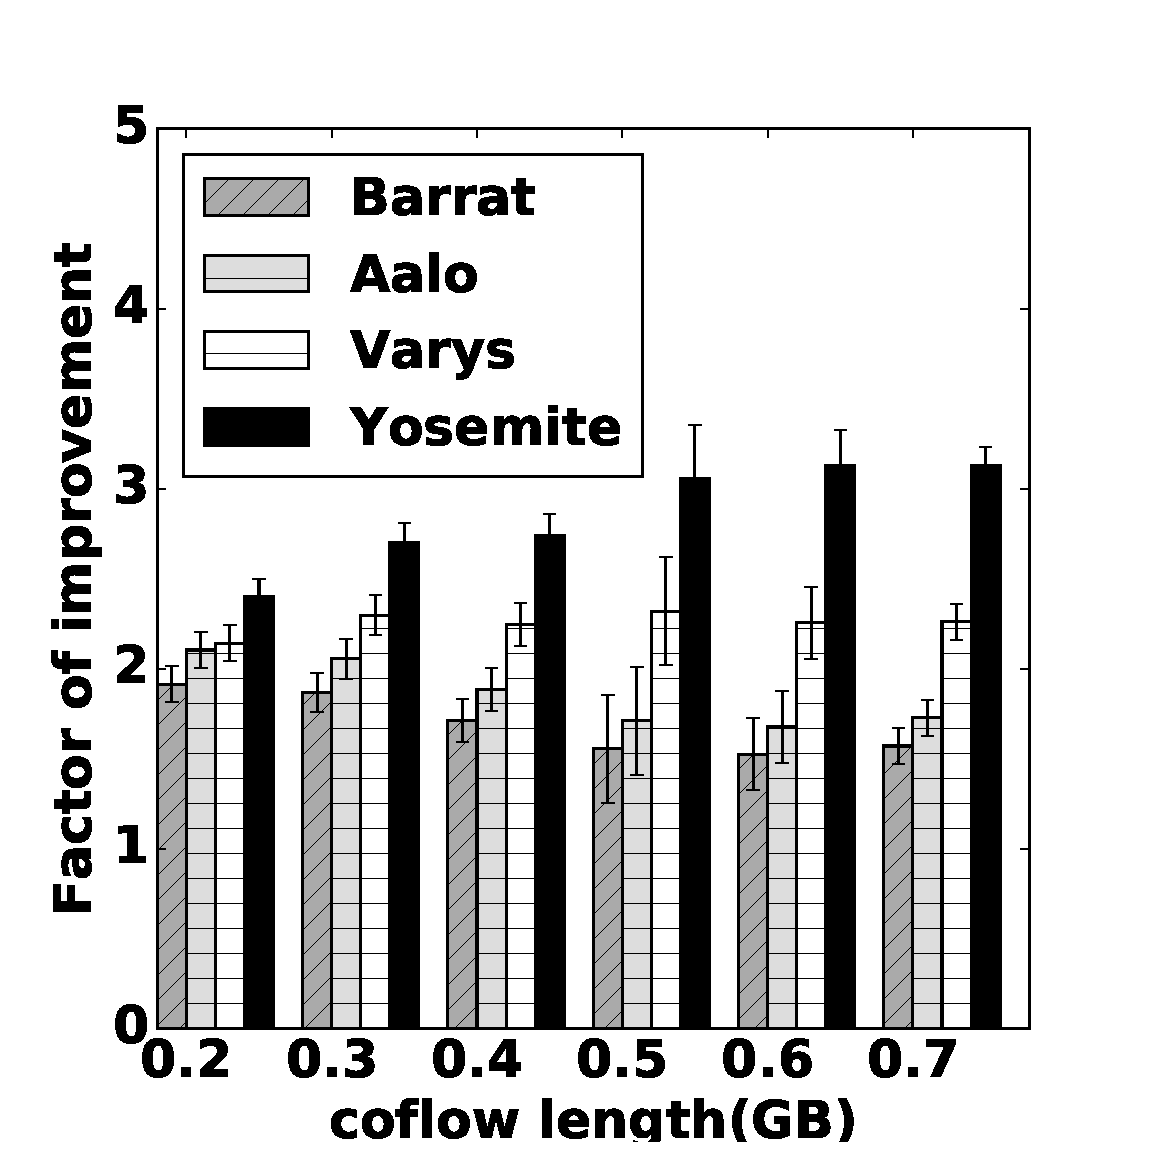
\includegraphics[width=1.65 in]{./figs/different/fraclength.eps}}
\hspace{0.1in}
\subfigure[Impact of coflow width] {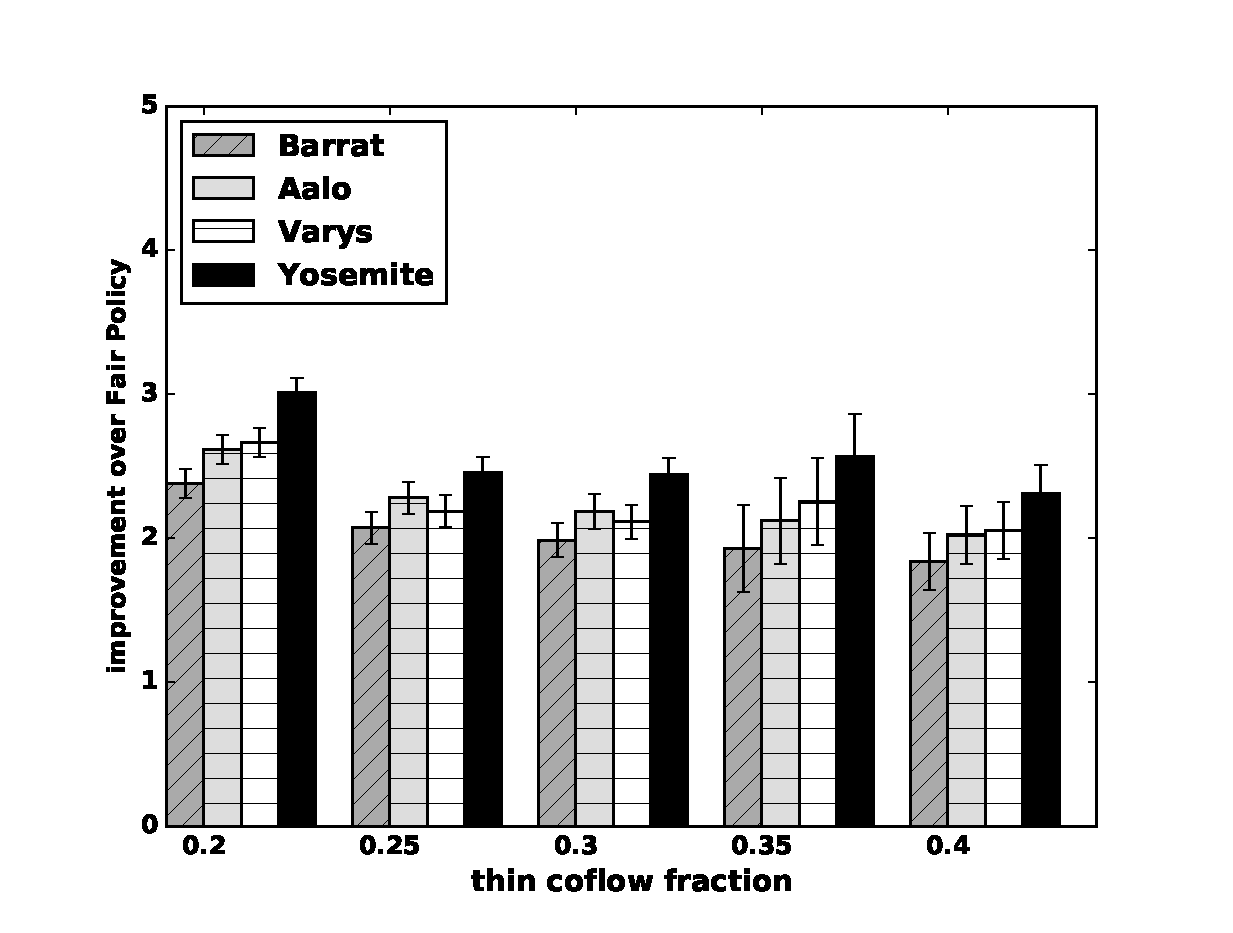
\includegraphics[width=1.65 in]{./figs/different/fracwidth.eps}}
\hspace{0.1in}
\subfigure[Impact of coflow weight] {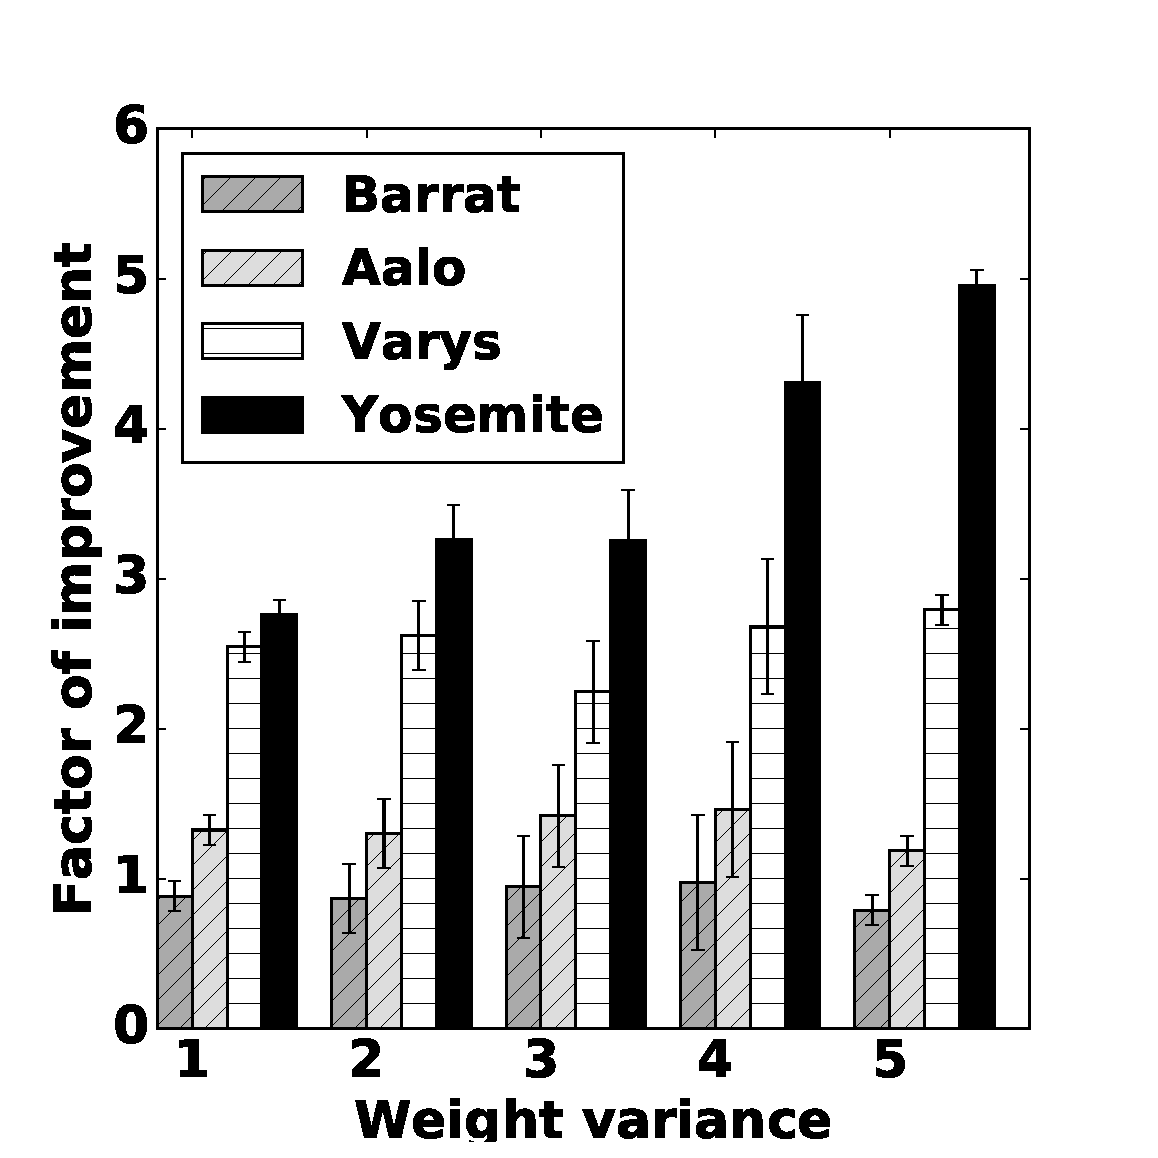
\includegraphics[width=1.65 in]{./figs/different/weight.eps}}
\vspace{-0.1 in}
\subfigure[Impact of coflow concurrency] {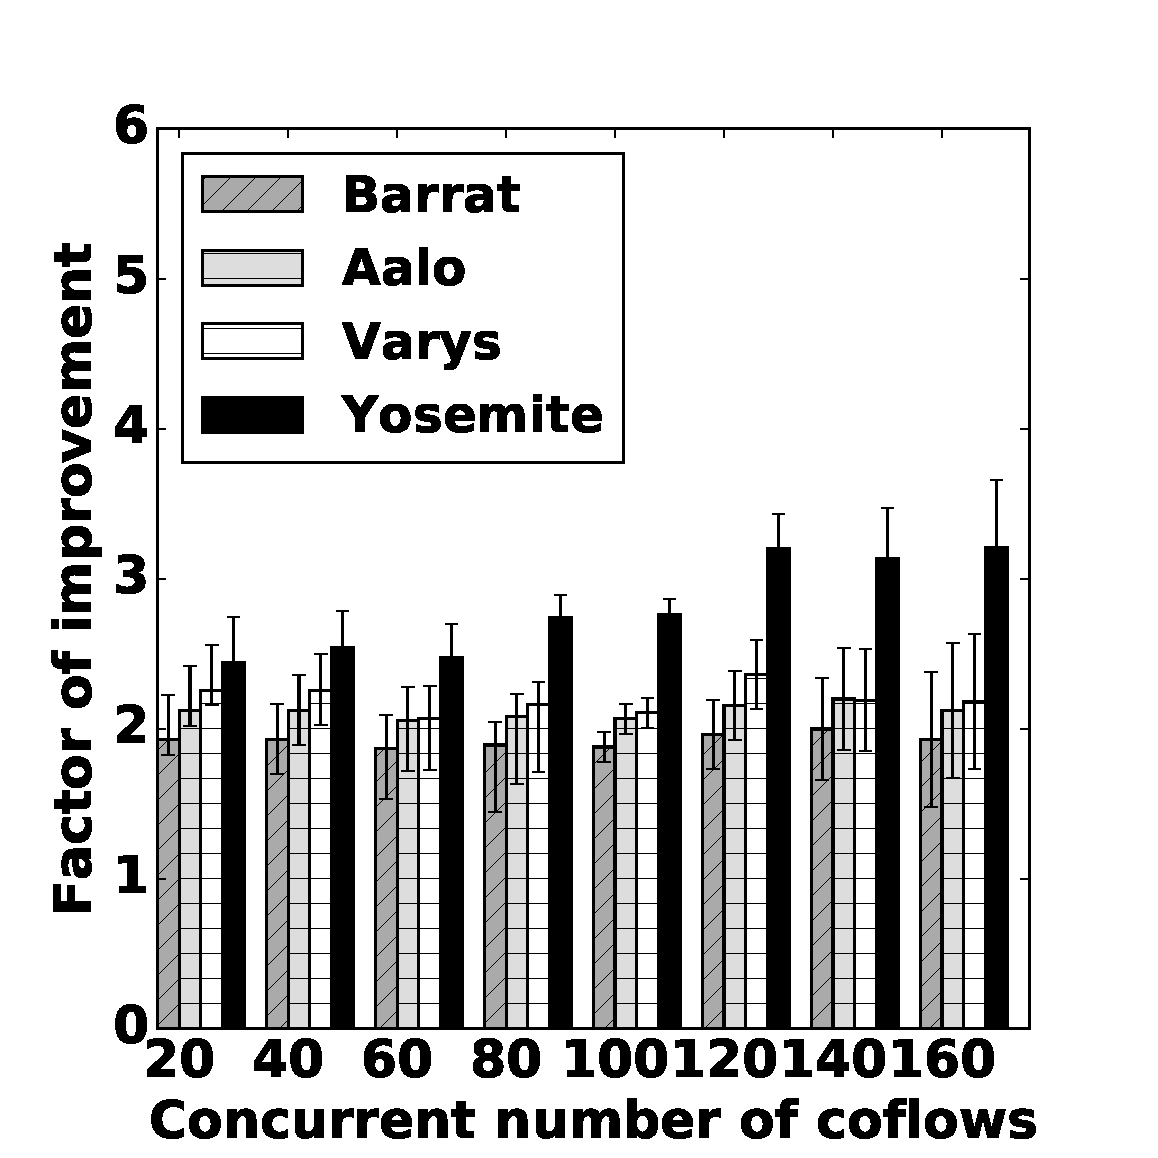
\includegraphics[width=1.65 in]{./figs/different/concurrent.eps}}
\caption{[Simulation] Yosemite performance comparison with Baraat and Varys, Aalo under different settings.}
\label{evalution_cases_different_fig}
\vspace{-0.1 in}
\end{figure*}
  \begin{figure}[b]
\begin{center}
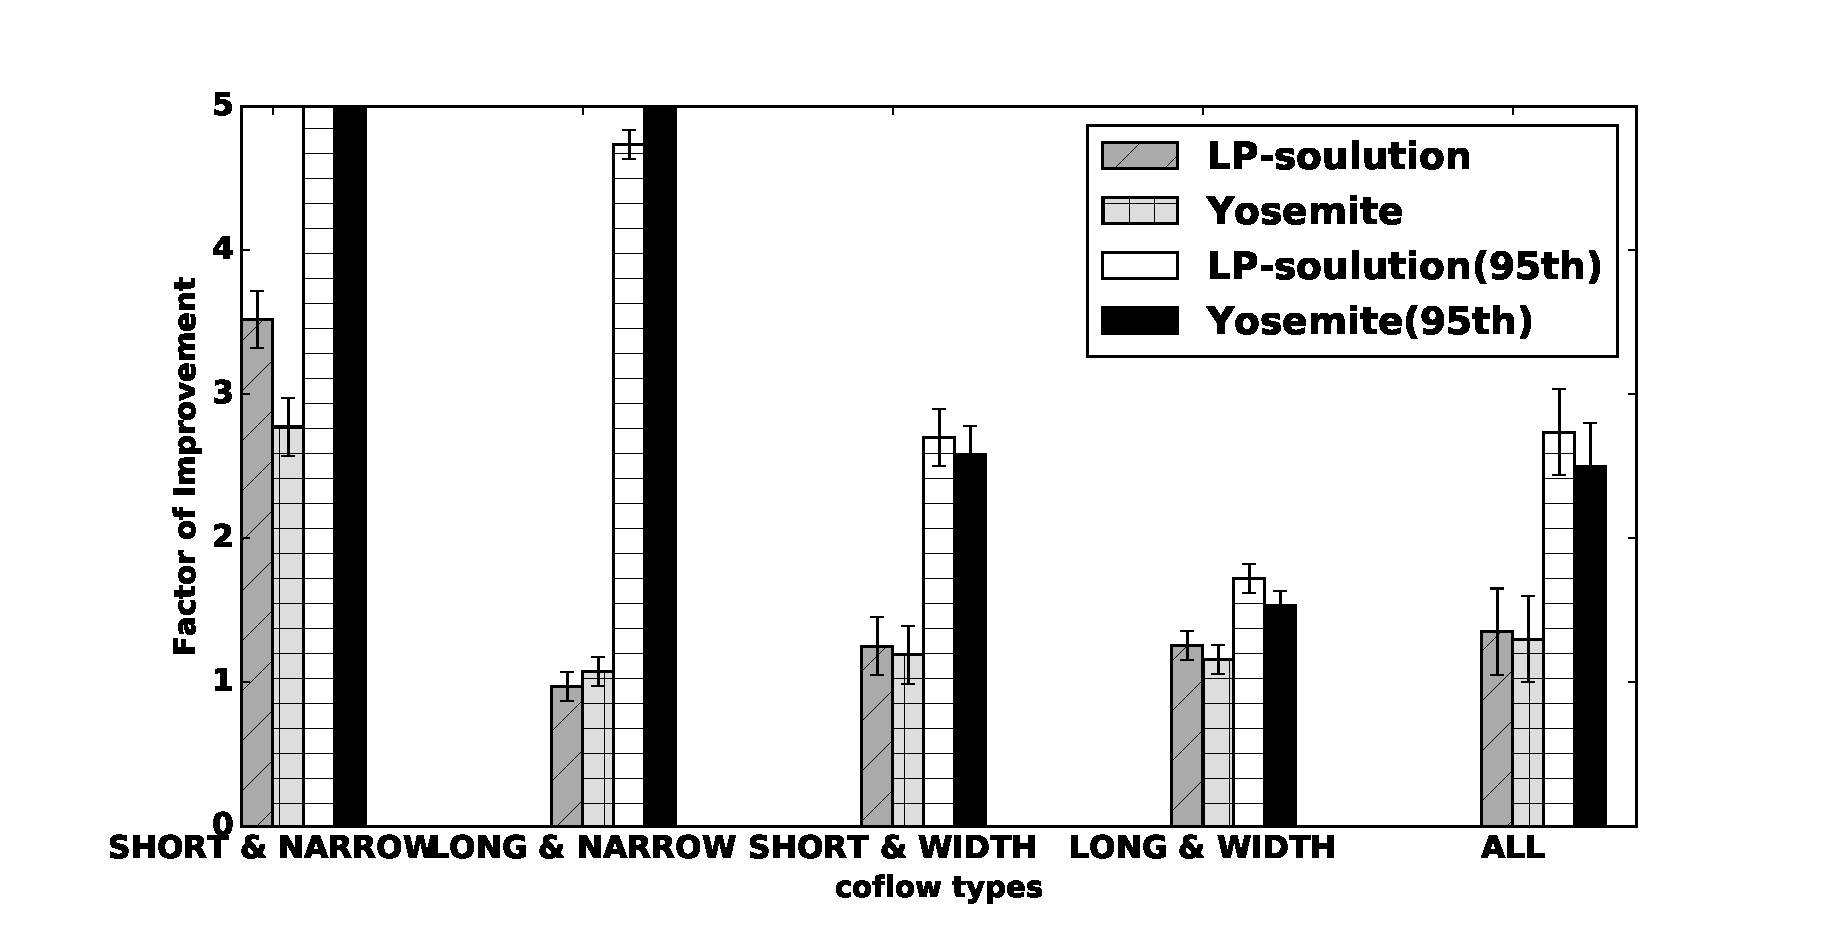
\includegraphics [width=1.0\columnwidth] {./figs/fake/fake1.eps}
\caption{ [Simulation] Performance comparison between the LP-based solution and Yosemite}
\label{LP-based-fig}
\end{center}
\end{figure}


\textbf{Open source}. To make our experiment repeatable, we publish main codes of Yosemite as well as Yosemite-Sim.
Sources of Yosemite can be downloaded at \cite{Yosemite}.
For larger scale of experiment in this paper, we use trace-driven simulation. 
Main codes of the Yosemite-Sim including trace generator can be downloaded at \cite{YosemiteSim}.
\subsection{Cloud platform evaluation} 
We deploy Yosemite at our private openstack platform which can start at most 80 virtual machines (2 Cores, 4GB Mem) simultaneously.
Operation system of each virtual machine is Ubuntu16.04. 
 With the help of Traffic Control module\cite{TC}, we constrain the maximum bandwidth of each VM's NIC to 1GB/s.
 
 Firstly, we run file distribute application to test the performance of Yosemite.
Each virtual node constantly construct files whose size ranging from 1KB to 200MB. 
Weight of each job is randomly generated ranging from 1 to 10.
Destinations are K nodes which are randomly chosen from the total nodes set.
Job can be regarded as finished until all the K nodes receive the file. 
TCP-fair is chosen as the baseline and Fig. \ref{distribute-fig} shows performance comparison between Yosemite and Varys. 
We repeat the process 10 times and the error bar indicates the max, min and average factor of improvement.
To decrease the influence of extreme values, we remove the top and last 2.5\% of each methods and recompute the factor of improvement, then we get
the 95th factor of improvement.
From  Fig. \ref{distribute-fig}, we can see in total, improvement factor of Yosemite is $3.1$ , while Varys is $2.1$.
Yosemite improves 30\% better than Varys. 
The 95th result shows Yosemite performs 31\% better than Varys, which is similar to Varys.

Work conserving aims to allocate the spare network resources to flows, as a result, network resources will be used more efficiently.
Efficient network utilization will accelerate the transfer process.
In Yosemite, scheduler allocates the spare bandwidth to flows equally to guarantee the utilization of network resources.
From Fig. \ref{conserving-fig} , we can see that with work conserving, factor of improvement of Yosemite is 2.1 in total, while that drops to 1.8 without work conserving. 

In reality, scheduler should be fast enough to compute out the scheduler order of coflows.
 Fig. \ref{overheads_fig}(a) shows the computation rate of Yosemite scheduler.
We can see for peak load, when active coflows is 140,  computation time of the scheduler is $\sim$23ms and
average computation time is less than 17ms. 
In our system, more than 90\% file transfers' time are more than 10s.
We think the average computation time is fast enough to get the schedule result.
Messages transferring between comm server is the main overheads of Yosemite system.
Error messages occurs when component crashes and server resources are insufficient.
As 80 VMs in our platform will reach full load, we start $1\sim 3$ dockers at each VM to get a slightly larger scale experiment.
Fig. \ref{overheads_fig}(b) shows the error messages frequency. 
We can see that when the concurrent worker number is over 200, peak error messages is over 4k/s.


Write down the trace of distribute file application and let the simulator run the trace under the same parameter.
Fig. \ref{sim-real} shows the performance gap between Yosemite and trace-driven simulator.
We can see performance gap between cloud platform and Yosemite is narrow($<15\%$).
In the following section, we use trace-driven simulator to test performance of Yosemite at larger scale.

\subsection{Trace-driven simulation} 
In this section, we use trace of facebook \cite{chowdhury2014efficient} to test the performance of Yosemite.
As the original trace doesn't include weight information, we randomly generate weight ranging from 1 to 10.
Repeat the process 100 times and Fig .\ref{evalution_real_weight_fig} shows the performance of Yosemite, Barrat, Varys,  Aalo and TCP fair-sharing. 
Note TCP fair-sharing is selected as the default baseline in this group.


 Fig. \ref{evalution_real_weight_fig}(a) implies that Yosemite greatly reduces the average weighted coflow completion time across all coflow types. 
 The improvement factors of Yosemite are 3.5 (Narrow\&Short), 1.6 (Narrow\&Long), 1.7 (Wide\&Short), 1.4  (Wide\&Long) and 1.5 (ALL), 
 while Varys are 2.4 (Narrow\&Short), 0.9 (Narrow\&Long), 1.2 (Wide\&Short), 1.3 (Wide\&Long) and 1.2 (ALL). 
 We repeat the experiment 100 times and error bar indicates maximum, minimum and average value. 
 To eliminate the  influence of extreme value, we we remove the top and last result 2.5\% of each methods and recompute the factor of improvement, then we get
the 95th factor of improvement.
 For the 95th case, we can find that Yosemite has the improvement factors on average weighted coflow completion time  of 30 (Narrow\&Short),20 (Narrow\&Long), 2.5 (Wide\&Short), 1.5  (Wide\&Long), and 2.5 (ALL), however Varys has 22 (Narrow\&Short),14 (Narrow\&Long), 2.1 (Wide\&Short), 1.2  (Wide\&Long) and 2.1 (ALL) and other 
 method such as Aalo and Barrat performs even worse than Varys.  
 Fig. \ref{evalution_real_weight_fig}(a) also indicates that FIFO\_LM based solution such as Barrat only accelerates the transmission of long tasks (including Narrow\&Long and Wide\&Long), however, for the short ones, it has poor performance. 
 This is because that FIFO\_LM based solution can lead to head-of-line blocking problem especially for the heterogenous coflows which has various flow length, width and arrival time.
 
 Fig. \ref{evalution_real_weight_fig}(b) is the distribution of wcct. 
 Compare with TCP-fair sharing method, through Yosemite can reduce average wcct, it prolongs the tail value. 
 That is to say, for applications which involves lot long flows, weighted completion time will have long duration using Yosemite and this is trivial for private cloud.
 
  Fig. \ref{evalution_real_weight_fig} indicates Yosemite can decrease wcct significantly. 
 One may be interested in the cct (coflow completion time) performance of Yosemite. 
 Fig. \ref{evalution_real_fig} shows cct performance of Yosemite, Barrat, Varys,  Aalo, TCP-fair sharing with the same settings, TCP-fair sharing is selected as the baseline. 
Fig. \ref{evalution_real_fig}(a) shows that the improvement factors of Yosemite on cct  are 2 (Narrow\&Short),1.1 (Narrow\&Long), 0.8  (Wide\&Short), 0.9   (Wide\&Long) and 1.3 (ALL) , while Varys performs about $\sim5\%$ better than Yosemite. 
 Fig. \ref{evalution_real_fig}(a) also shows the maximum value and minimum value of Yosemite under different weight settings. 
 For Barrat, Aalo and Varys, as their cct have no relationships with weight, so that average cct  will not change under different weight settings.  
 Fig. \ref{evalution_real_fig}(b) shows the result of distribution of coflow completion time which is similar to Fig. \ref{evalution_real_weight_fig}(b).
 
 
 \subsection{Performance under different settings} 
 In this section, we explore the performance of Yosemite under different settings. 
From Algorithm \ref{online-algorithm},  we can see performance of Yosemite is mainly influenced by coflow length, coflow width, coflow weight and coflow concurrency. 
 In this part, we explore Yosemite's performance from the four aspects.
 
 \begin{table}[!htb]
          \centering
          \footnotesize
          \caption{Default parameters in each group of experiment} \label{tab:parameters}
          \begin{tabulary}{\textwidth}{cccccr}
              \toprule
               Number &Length & Width & Weight & Arrival&Capacity\\
              \midrule
              \multicolumn{1}{r}{512}&[100KB,10GB]   &60& [1,10]  & [0s,1000s]&10GB/s\\
              \bottomrule
          \end{tabulary}
      \end{table}
      
 
In each group of experiment, we fix the value of other parameters and only change the factor we want to study. 
Table \ref{tab:parameters} shows the default settings of parameters. 
We start 512 coflows in each group of experiment and length of each coflow are within 100KB to 10GB. 
Width of each coflows are at most 60 and weight of each coflows are within 1 to 10. 
coflow's arrival time ranges 0s to 1000s. 
Ingress and egress port capacity in our experiment are 10GB/s. 
We repeat each group of experiments 100 times and draw maximum, minimum as well as average value pictures.

 \subsubsection{Impact of coflow length}
 In this group of experiment, we test the influence of coflow length.
 Coflow width, weight, arrival time are set as Table \ref{tab:parameters} shown. 
 In each group of experiment, we only change length of coflow.  
 Coflow length in our experiment are set within [100KB,K]. 
 Varying K from 1GB to 6GB. 
 Fig. \ref{evalution_cases_different_fig}(a) shows the result. 
 From Fig. \ref{evalution_cases_different_fig}(a) we can see that with the increasing of K, improvement of Yosemite becomes larger. 
 For example, when K is 1GB,  improvement of Yosemite is 2 and when K is 6GB, improvement of Yosemite is 3. 
Indeed, when K becomes larger, length differentiation between coflows becomes larger, scheduling result is better.
 
 \subsubsection{Impact of coflow width}
Fig. \ref{evalution_cases_different_fig}(b) shows the influence of coflow width.  
In this group of experiment, we vary the fraction of thin coflows (width$<$ 30) from 20\% to 40\%.
Coflow length, width, as well as coflow arrival time are set as Table \ref{tab:parameters} shown. 
From  Fig. \ref{evalution_cases_different_fig}(b), we can see that with the increasing fraction of thin coflows,  improvement of Yosemite becomes smaller.  
The reason for this is that, when fraction of thin coflows is small, conflict probability between coflows is large, so it is necessary to decide a suitable scheduling sequence of coflows.
 
 \subsubsection{Impact of coflow weight}
 Weight indicates the importance of the application in reality. 
 Weight setting has huge influence on the performance of weighted coflow completion time. 
 In this section, we study the influence of weight. 
 Coflow length, width and arrival time are set according to Table \ref{tab:parameters}.
Weight are generated within $[8-\sigma,8+\sigma]$, varying $\sigma$ from 1 to 5 and
Fig. \ref{evalution_cases_different_fig}(c) shows the result. 
From Fig. \ref{evalution_cases_different_fig}(c), we can see that when weight variance $\sigma$ becomes larger, improvement of Yosemite becomes larger. 
This means Yosemite works better for larger weight variance cases.
 
 \subsubsection{Impact of coflow concurrency}
In real word, coflow can start at any time. 
Arrival time of coflows can impact the traffic load in data center network. In this part, we explore the impact of coflow concurrency. 
Changing the number of coflows that start at time 0. 
Fig. \ref{evalution_cases_different_fig}(d) shows the result. 
We can see that with the concurrent number of coflows increasing, improvement of Yosemite becomes larger.  
The reason for this is that when workload becomes heavier, the optimization space for preemptive scheduling become larger.
  
  \subsection{Distance to Optimization}
 
It is hard to find the optimal schedule, so that we find an LP-based solution \cite{qiu2015minimizing} whose approximation ratio is
$\frac{67}{3}$ to compare with. 
Use facebook trace and generate weight within 1 to 5, then repeat the experiment 20 times and Fig. \ref{LP-based-fig} shows the result. 
We can see that Yosemite has less than 10\% performance gap.
 
 \section{Conclusion} \label{conclusion}
 In this paper, we use weight to quantify the importance of applications.  
Coflows belonging to important applications own large weight.
We design and implement Yosemite-a coflow scheduling system that aims to minimize average weighted coflow completion time.
We test the performance of it by trace-driven simulation and test-bed deployment.
Experiments show Yosemite can reduce average weighted coflow completion time significantly.  

Although Yosemite works well on minimizing average weighted coflow completion time, it is clairvoyant method.
Indeed in data center network, applications such as file backup, file distributes can know coflow details, but for some computation applications, they are hard to get.
To make Yosemite use more widely, in the future, we will make advance of Yosemite to let it work in non-clairvoyant way.


\bibliographystyle{abbrv}
\bibliography{paper}



\end{document}



